%吉野君
\usepackage{here}

\title{ビッグデータ処理技術を用いた\\
Wikipediaマイニング}
\author{プロジェクトマネジメントコース\\
ソフトウェア開発管理グループ\\
矢吹研究室\\
1242005\\
石井康之}
\date{}
\begin{document}
\maketitle

%本テンプレートの余白は,卒論マニュアルで指示されたものとは違っているが,1ページあたりの文字数は40文字x40行と,卒論マニュアル通りになっている。文字間隔や行間隔を調整して,余白をマニュアル通りにすることもできるが,それでは文章が読みにくくなるため,このような対応をしている。

%\noindent
□□□□□□□□□■□□□□□□□□□■□□□□□□□□□■□□□□□□□□□■
□□□□□□□□□■□□□□□□□□□■□□□□□□□□□■□□□□□□□□□■
□□□□□□□□□■□□□□□□□□□■□□□□□□□□□■□□□□□□□□□■
□□□□□□□□□■□□□□□□□□□■□□□□□□□□□■□□□□□□□□□■
□□□□□□□□□■□□□□□□□□□■□□□□□□□□□■□□□□□□□□□■
□□□□□□□□□■□□□□□□□□□■□□□□□□□□□■□□□□□□□□□■
□□□□□□□□□■□□□□□□□□□■□□□□□□□□□■□□□□□□□□□■
□□□□□□□□□■□□□□□□□□□■□□□□□□□□□■□□□□□□□□□■
□□□□□□□□□■□□□□□□□□□■□□□□□□□□□■□□□□□□□□□■
□□□□□□□□□■□□□□□□□□□■□□□□□□□□□■□□□□□□□□□■
□□□□□□□□□■□□□□□□□□□■□□□□□□□□□■□□□□□□□□□■
□□□□□□□□□■□□□□□□□□□■□□□□□□□□□■□□□□□□□□□■
□□□□□□□□□■□□□□□□□□□■□□□□□□□□□■□□□□□□□□□■
□□□□□□□□□■□□□□□□□□□■□□□□□□□□□■□□□□□□□□□■
□□□□□□□□□■□□□□□□□□□■□□□□□□□□□■□□□□□□□□□■
□□□□□□□□□■□□□□□□□□□■□□□□□□□□□■□□□□□□□□□■
□□□□□□□□□■□□□□□□□□□■□□□□□□□□□■□□□□□□□□□■
□□□□□□□□□■□□□□□□□□□■□□□□□□□□□■□□□□□□□□□■
□□□□□□□□□■□□□□□□□□□■□□□□□□□□□■□□□□□□□□□■
□□□□□□□□□■□□□□□□□□□■□□□□□□□□□■□□□□□□□□□■
□□□□□□□□□■□□□□□□□□□■□□□□□□□□□■□□□□□□□□□■
□□□□□□□□□■□□□□□□□□□■□□□□□□□□□■□□□□□□□□□■
□□□□□□□□□■□□□□□□□□□■□□□□□□□□□■□□□□□□□□□■
□□□□□□□□□■□□□□□□□□□■□□□□□□□□□■□□□□□□□□□■
□□□□□□□□□■□□□□□□□□□■□□□□□□□□□■□□□□□□□□□■
□□□□□□□□□■□□□□□□□□□■□□□□□□□□□■□□□□□□□□□■
□□□□□□□□□■□□□□□□□□□■□□□□□□□□□■□□□□□□□□□■
□□□□□□□□□■□□□□□□□□□■□□□□□□□□□■□□□□□□□□□■
□□□□□□□□□■□□□□□□□□□■□□□□□□□□□■□□□□□□□□□■
□□□□□□□□□■□□□□□□□□□■□□□□□□□□□■□□□□□□□□□■
□□□□□□□□□■□□□□□□□□□■□□□□□□□□□■□□□□□□□□□■
□□□□□□□□□■□□□□□□□□□■□□□□□□□□□■□□□□□□□□□■
□□□□□□□□□■□□□□□□□□□■□□□□□□□□□■□□□□□□□□□■
□□□□□□□□□■□□□□□□□□□■□□□□□□□□□■□□□□□□□□□■
□□□□□□□□□■□□□□□□□□□■□□□□□□□□□■□□□□□□□□□■
□□□□□□□□□■□□□□□□□□□■□□□□□□□□□■□□□□□□□□□■
□□□□□□□□□■□□□□□□□□□■□□□□□□□□□■□□□□□□□□□■
□□□□□□□□□■□□□□□□□□□■□□□□□□□□□■□□□□□□□□□■
□□□□□□□□□■□□□□□□□□□■□□□□□□□□□■□□□□□□□□□■
■■■■■■■■■■■■■■■■■■■■■■■■■■■■■■■■■■■■■■■■
□□□□□□□□□■□□□□□□□□□■□□□□□□□□□■□□□□□□□□□■%文字数チェック用

\chapter*{謝辞}

本研究を進めるにあたり,矢吹研究室矢吹太朗准教授には,多くの時間をご指導にさいて頂きました.
また矢吹研究室の皆様には,多くの知識や示唆を頂きました.協力していただい皆様に感謝の気持ちと御礼を申し上げます.

\tableofcontents%目次

\chapter{序論}

Wikipediaは,多くの人がボランティアで執筆するオンライン百科事典プロジェクトである.

Wikipediaは2001年1月15日に創設され,2001年5月ごろに日本語版が発足した.

多くの人が参加するプロジェクトの代表例であるWikipediaを調査することによって,このような形式のプロジェクトのマネジメントについての有意義な知見が得られることが期待できる.

このオープンなオンライン百科事典プロジェクトの成功理由について様々な考察がされており,その中の1つの要因に「適切な時に,それぞれのニッチに対しボトムアップとトップダウンの適切な混合率を出していた」というのがある\cite{bottom1}.
Wikipediaでは,ボトムアップの力,無統制の善良さで成長したと見えるのだが,実際にプロセスをよく調べてみると,見かけ以上に入念なトップダウンのしくみによる管理がなされている.

Wikipediaの編集者の中には,管理者と呼ばれる利用者たちがおり,この利用者たちが統制を行っているのではないかと考えた.

そこで当研究では,管理者の動向を見るため,管理者の編集回数がどのように変化しているか調査する.結果からWikipediaの成功理由に,この管理者がどのように関係しているか見つけ出す.



\chapter{背景}

\section{研究背景}
Wikipediaは,多くのボランティアにより,始まってから10年足らずの間に,大きな成長を見せたオンライン百科事典プロジェクトである.総記事数の文字数は10億文字を超え,ブリタニカ国際大百科事典とエンカルタ総合大百科の合計と比較しても上回る.Wikipediaは,さまざまな言語が参加しているグローバルなプロジェクトでもある.2015年9月までには,291個もの言語が参加している.

このオープンなプロジェクトの百科事典は,制限無く誰でも自由に使用でき編集することもできる.

誰でも自由に編集できるからこそ,ボランティアの人々は気軽に参加でき,特定の企業や個人のお金を稼ぐのに力を貸していると感じることなく,時間と労力を注ぐことができる.

記事の内容はボランティアの人々の協力によって,信頼のおける品質が保たれている.しかし,中には協力的では無く,悪意のある編集をするものがいる.悪意のある編集者はその記事の内容とは関係ないことを書き込んだり,記事の破壊行為を繰り返している.Wikipediaでは,悪意のある編集をする人とわかっていても規制などをしたりはしない.記事は完成・確定されることはなく,新しい情報にいつでも改変することができる.

本研究では,Wikipediaの全編集データをマイニングすることによって,Wikipediaの品質が保たれている理由を見つけ出す.


\chapter{Wikipedia}

\section{Wikipediaとは}

フリー・ライセンスの百科事典である.フリーには2つの意味がある.無料という意味と,自由という意味だ.Wikipediaのフリーは後者の自由という意味であり,四つの自由が与えられている.著作物を複製する自由.改変する自由.再頒府する自由.そして,改変版を再頒府する自由だ.そして,営利目的に使っても,非営利に使ってもかまわない.というものがある.Wikipediaがフリーの百科事典であるというのは,無料でアクセスできるということではなくて,自由に複製,改変,利用してかまわないということである.

Wikipediaという名前は,ウェブブラウザ上でウェブページを編集することができるWikiというシステムを使用した百科事典であることに由来する造語である.設立者の1人であるラリー・サンガーにより命名された.

Wikipediaは2015年9月までには,291個もの言語が参加している.この百科事典は多くの言語のボランティアたちによって書かれたグローバルなプロジェクトでもある.\cite{wikirevo}

Wikipediaは10年足らずの間に,百科事典の世界を活発化させ,激変させた.インターネットを利用する誰もが日々何気なくコンテンツにアクセスするまでになった.それでも,Wikipediaが身元も知らない多くのボランティアによって無償で作成されていることを知っている利用者は少ない.

Wikipediaの各記事には「編集」ボタンがあり,通りがかりの匿名ユーザでさえも,好きな記事の内容を編集できる.「ユーザ生成コンテンツ」を取り入れている多くのインターネット・サイトとは異なり,Wikipediaの変更には,登録やメールアドレス,認証などは必要としない.「誰でも編集できる」モデルというと,手に負えない無秩序や暖混乱,荒らしなどが生まれると思われるが,そういった予想とは逆に,高い人気や評価を誇るオンライン百科事典が築き上げられた.無数のボランティアたちが,自主的にオンライン・コミュニティを作成し,想像を超える成功を収めてきた.その結果,Wikipediaは多くの人々が頼りにするサイトとなり,現在ではインターネット上での根幹を担っている.

\section{成功したといわれる色々な要因}

Wikipediaが成功した要因となったのは,シンプルな原則があげられる.ハッカー文化に基いて、フリーで,オープンで,中立的で,リアルタイムで,社会的な百科事典の作成方針を築いた.

Wikipediaでは,誰もが自由に編集することが出来る.コミュニティのメンバーが任意のアクションを簡単に取り消すことができるため,誰もが気軽に編集することができる.破壊よりも修復の方が簡単なのである.荒らしが不正な情報を大量に流そうとしても,他のユーザーがすばやく簡単に阻止することができる.この性質は,生産的で協力的なコミュニティのメンバーにとっては都合がよく,その結果品質の高いコンテンツが広まることになった.

Wikipediaのプロジェクトの執筆方法として,完全にオープン性である.透明性が重視されており,あらゆる内容がコミュニティ内で監視されている.また,各記事は作成時からのあらゆる変更が年代順に記録されており,ユーザーの活動はすべてのシステムに詳細に記録され,誰もが追跡できるようになっている.その結果,お互いに共有を行えるようになり,作業を監視したり,賞賛したり,学んだり,問題を提起したり,協力したり出来る.


また,Wikipediaでは「完全な中立性」も成功要因の1つである.数多くの人が共同で何かを築き上げるためには,中心的な編集方針として「中立性」欠かせないからである.例えば,何かの問題が出て,支持者と反対者が出たとき,両者とも同意できる形で記述するということだ.インターネット上の人々が共同で様々な観点や背景を持つ人々をまとめなければならない.そこで,Wikipediaでは,創始者が思想の違いによってサイトが分裂しないように「敵対作業ではなく共同作業」を原動力にしようと考えた.完全な中立性を実現することは不可能かもしれないが,コミュニティは,特定の話題を統一的に扱うという理想的なビジョンをもち一致団結していき,この方針は非常に有効だった.



Wikipediaの上を行くGoogle,Yahooといったウェブサイトは,いずれも数万人の従業員を抱える数十億ドル規模規模の企業である.一方で,Wikipediaの運営予算は50万ドルにも満たず,有給従業員は数名ほどしかいない.





\section{記事の編集の仕方}

 一部の保護されているページを除いて,全てのページには「編集」と書かれたリンクがあり,このリンクを使って,あなたが閲覧しているページを編集することができます.編集ができることはウィキペディアの大きな特徴で,この機能を使って,あなたが記事を修正したり,記事に加筆することができるのです.記事に情報を加筆する時には,情報の出典を明記してください.出典が不明な記述は,除去の対象となります.\cite{wikiEdit}

%図の挿入
\begin{figure}[H]
\centering
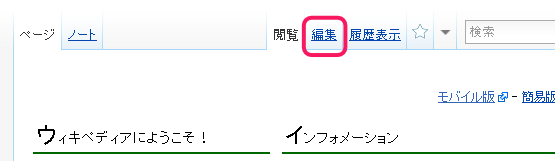
\includegraphics[width=13cm]{sample1.png}
\caption{編集の仕方1}\label{サンプル図}
\end{figure}

これから常に使ってほしい大切な機能が「プレビューを表示」ボタンです.サンドボックスでなにか編集をして,それから「以上の記述を完全に理解し同意した上で投稿する」ボタンではなく,「プレビューを表示」ボタンを押してみましょう.そうすると,あなたがページに加えた変更の結果を,実際に保存する前に確認することができます.間違いは誰にでもあります.この機能は,間違いがないか自分で確認するためのものです.また,「プレビューを表示」ボタンを使えば,試しにページの体裁や表現をいろいろと変えてみても,ページの変更の記録にいちいち記録されずにすみますし,他にもいろいろと利点があるのです.でも,プレビューをした後,最後には保存するのを忘れないでください.\cite{wikiEdit}

%図の挿入
\begin{figure}[htb]
\centering
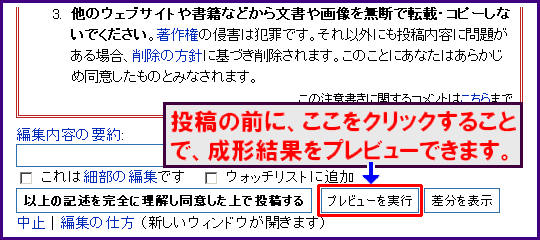
\includegraphics[width=13cm]{sample2.png}
\caption{編集の仕方2}\label{サンプル図}
\end{figure}

「以上の記述を完全に理解し同意した上で投稿する」ボタンを押す前に、あなたが行った編集の説明を、編集用のテキストボックスと保存ボタンの間にある要約欄に書き込むようにしましょう。ウィキペディアでは、ここに編集の説明を書き込むことが大切なエチケットと考えられています。ただ単に誤字を直したような時には「誤字修正」と書けば充分です。文章の意味に影響を及ぼさないような、小さな修正のときには、要約欄の下にある「これは細部の編集です(説明)」のチェックボックスにチェックをいれておいてください(この機能はログイン時にのみ有効です)。\cite{wikiEdit}

%図の挿入
\begin{figure}[htb]
\centering
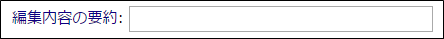
\includegraphics[width=13cm]{sample3.png}
\caption{編集の仕方3}\label{サンプル図}
\end{figure}

\subsection{Wikipediaの編集履歴データ}

データCreative Commons Attribution-ShareAlike 3.0 Unported License (CC-BY-SA) および GNU Free Documentation License (GFDL) の下にライセンスされており (Wikipedia:著作権および利用規約を参照),再配布や再利用のためにデータベース・データの提供が行われています.データの生成は不定期に行われている.

Wikipediaではクロール行為のデータダウンロードは禁止されている.強引なクローリングは,Wikipediaが劇的に遅くなる原因となってしますためである.データベースから自動的にデータ収集している行為が発券された場合、システムの管理者から自身のサイトからWikipediaのアクセスを禁止されてしまう措置が起こってしまうこともある.また,ウィキペディア財団が法的措置を検討する場合もあるので,注意が必要.

%図の挿入
\begin{figure}[htb]
\centering
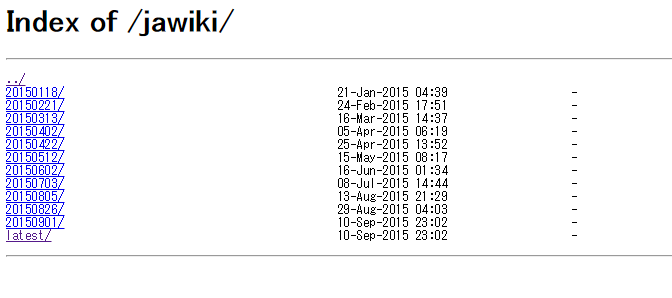
\includegraphics[width=13cm]{sample4.png}
\caption{Wikipedia dump}\label{サンプル図}
\end{figure}

ここに日本語版Wikipediaの履歴データが記録されている.

{\small
\begin{verbatim}
https://dumps.wikimedia.org/jawiki/
\end{verbatim}}



他の言語もこのような形式で履歴データが残されている.他の言語のデータを取得したい場合はURLのhttps://dumps.wikimedia.org/○○wiki/の○○の部分を変更すればよい.言語は英語のスペルで頭文字2文字でよい.

例:英語の場合はスペルはEnglishなので,https://dumps.wikimedia.org/enwiki/とすればよい.



%図の挿入
\begin{figure}[H]
\centering
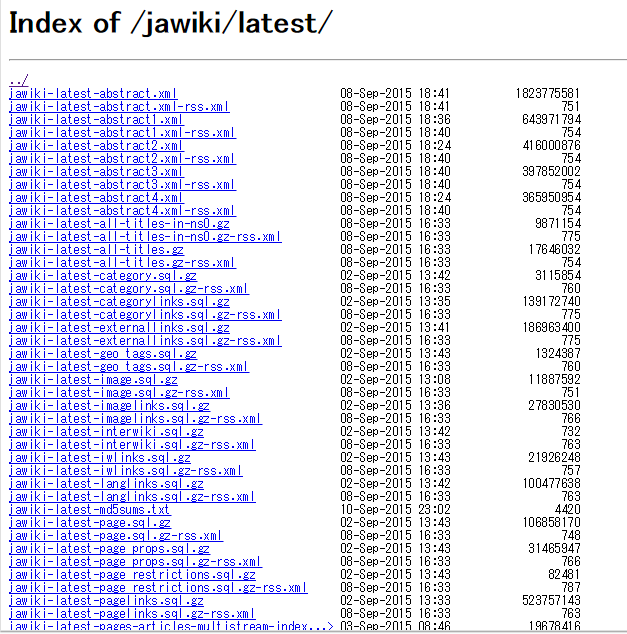
\includegraphics[width=13cm]{sample5.png}
\caption{日本語版Wikipediaの編集履歴データ}\label{サンプル図}
\end{figure}

どれか開くと上記のような画面になる.\\
ウィキページのデータはSQLのテーブルではなく、XMLで提供されている。XMLファイルの文字エンコーディングはUTF-8である。 非常にファイルサイズが大きいため、通常のエディタやブラウザで、解凍してはいけない。\\
データの詳細は下記のとおり

\begin{itemize}
 \item pages-articles.xml.bz2 - ノートページ、利用者ページを除く最新版のダンプ
 \item pages-meta-current.xml.bz2 - 全ページの最新版のダンプ
 \item pages-meta-history.xml.7z - 全ページの全ての版のダンプ
 \item all-titles-in-ns0.gz - 全項目のページ名一覧 (標準名前空間)
\end{itemize}


%次のページに移動
\clearpage


\section{Wikipediaの編集回数の多いページの一覧}

期間: 2014-07-01 — 2014-07-31 のランキング.


%図の挿入
\begin{figure}[H]
\centering
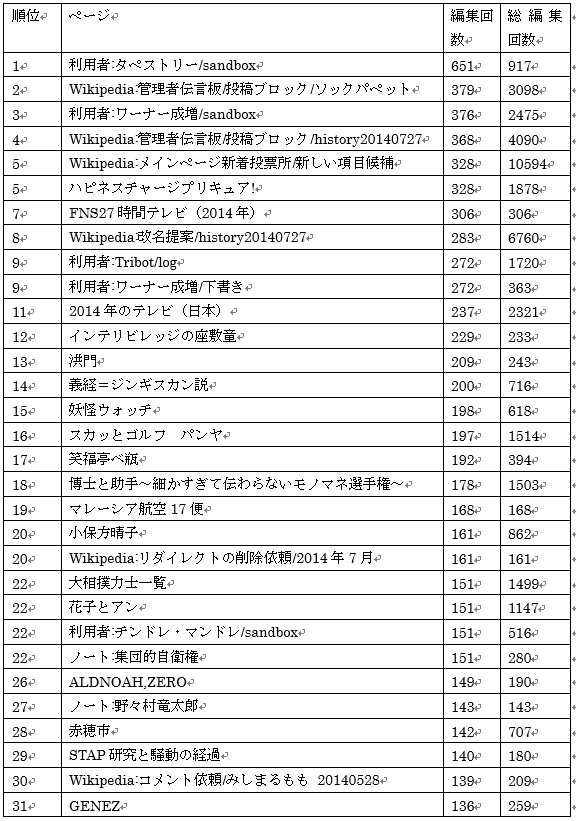
\includegraphics[width=12cm]{sample6.png}

\end{figure}


%図の挿入
\begin{figure}[H]
\centering
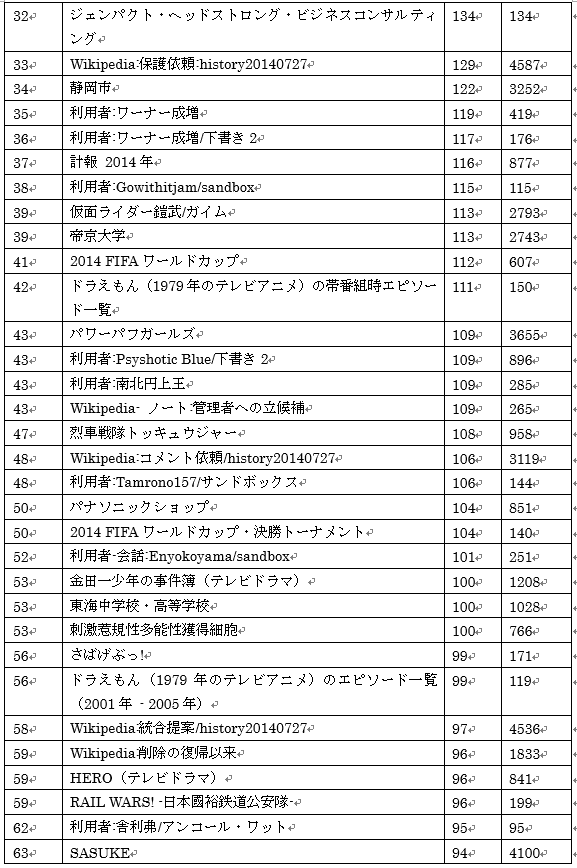
\includegraphics[width=12cm]{sample7.png}

\end{figure}


%図の挿入
\begin{figure}[H]
\centering
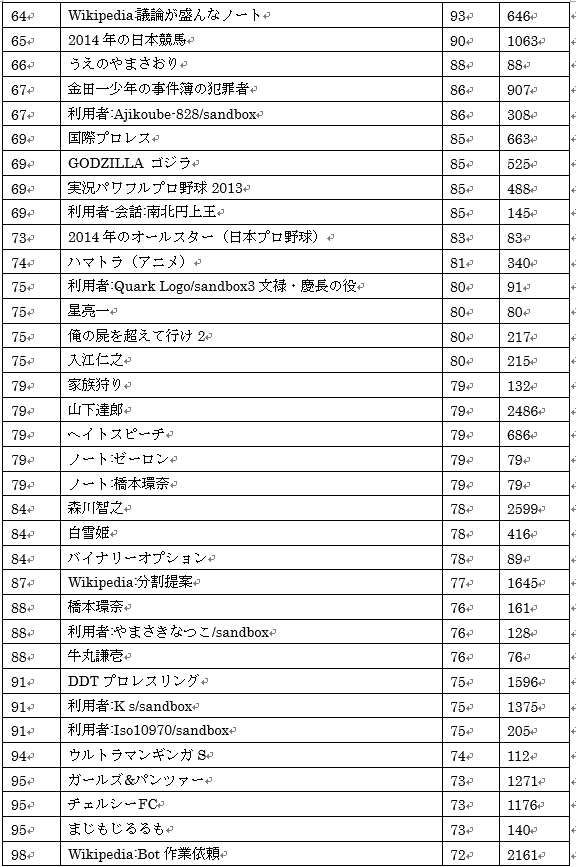
\includegraphics[width=12cm]{sample8.png}

\end{figure}


%図の挿入
\begin{figure}[H]
\centering
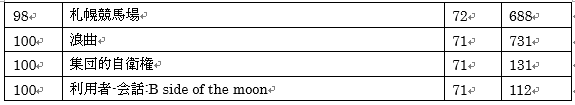
\includegraphics[width=12cm]{sample9.png}

\end{figure}


\section{日本語版Wkipediaについて}

日本語版のWikipediaは,英語版Wikipediaと比べると非常にユニークに見える.まず編集者として行動するときに,日本のウィキペディア編集者は,匿名が多い.これは元々ネットを使うことにおいて匿名でいるが多い日本のインターネット文化が大きな要因である.日本のオンライン活動に大きな影響を与えているサイトに,「2ちゃんねる」というものがある.2ちゃんねるは,匿名の投稿で有名なサイトである.日本のウィキペディア編集者あえてユーザー登録をしない理由のひとつとして,自分の身元を明かさない2ちゃんねるの「完全な匿名性」の普及が上げられることが多いといえる.

また,日本語版ウィキペディアの編集者は,英語版のような激しい編集合戦はあまり行われない傾向がある.礼儀正しい日本の文化では,長きにわたって繰り広げられる卑劣な論争は,一般的に社会には受け入れられないからだ.日本のユーザーは欧米と比べるとおとなしい.公開された既存の記事を思い切って変更などもしない.代わりに,他の場所やノート・ページで別のバージョンを考えることが多い.

日本語版ウィキペディアの欠点は,登録ユーザーが少ないことだ.先ほどでも挙げたとおり,匿名性の普及が多いことが要因といえる.登録ユーザーの数が少ないので,ウィキペディア・ユーザーの国際コミュニティや,全プロジェクトを取りまとめる非営利のウィキペディア財団への参加が少ないという問題がある.

日本語版ウィキペディアの規模はトップクラスであるが,2005年にフランクフルトで開催された第一回のウィキペディア会議のウィキマニアでは,日本人の登録参加者は二名だけたっだ.日本語版よりも小規模なフランス,ポーランド,オランダや,さらに小規模な中国でさえ,日本語版ウィキペディアよりも多くの代表者が参加していた.このことから,日本語版ウィキペディアの欠点はやはり登録しているユーザーが少ないということがあげられる.



%次のページに移動
\clearpage


\subsection{実装してから2015年9月までの月毎の編集回数}

%図の挿入
\begin{figure}[H]
\centering
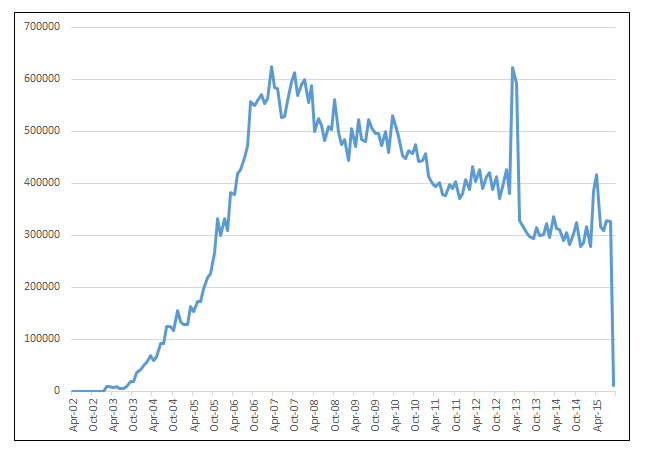
\includegraphics[width=10cm]{month1.png}
\caption{月別編集回数}\label{サンプル図}
\end{figure}

日本語版Wikipediaの月毎の編集回数.2006年の6月まで順調に伸び続けていた.それからは少しずつだが編集回数が減少して言っている傾向が見える.2013年の3月と4月において,前のつきの2月と比べると倍以上の編集回数に伸びていたので,その月にどんな記事が頻繁に編集が行われていたか調査した.

%図の挿入
\begin{figure}[H]
\centering
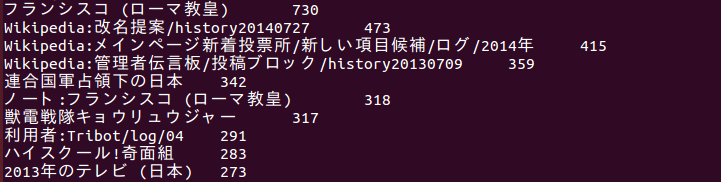
\includegraphics[width=12cm]{revision2013_03.png}
\caption{2013年3月の編集回数ランキング}\label{サンプル図}
\end{figure}

最も多く編集が行われていた記事は「フランシスコ(ローマ教皇)」という記事だった.調べてところ2013年3月13日に,ローマ教皇が新しい人に変わっていたことが分かった.このことが要因で編集回数が伸びたと考えた.



\chapter{ビッグデータ}

\section{ビッグデータとは}

パソコン,スマートフォンが普及し「ビッグデータ」という言葉が流行することからもわかるように,私たちは膨大な情報を日々生み出しながら生活している.GoogleやYahoo!に寄せられる大量の検索クエリや,Twitter,FacebookなどのSNSに投稿される文章や画像,動画,スマートフォンを利用するサービスなどで収集される位置情報データ,防犯カメラで記録される人間の表情や動きのデータなどの膨大な量のデータを指す.

ビッグデータとは,一般的にペタ(1,000兆),バイト級のデータ量といわれている.このような数値的定義もあるが,ペタバイト以下であればビッグデータではないという訳でもなく,本質的には,「従来の手段では管理しきれない規模のデータ」を指す.

\begin{table}[H]
  \begin{tabular}{|c|c|c|c|l|c|} \hline
    $10^n$ & 接頭辞 & 記号 & 漢数字表記 & 十進数表記 & 分類 \\ \hline
    $10^21$ & ゼタ(zetta) & Z & 十垓 & 1,000,000,000,000,000,000,000 & ビッグデータ \\ \hline
    $10^18$ & エクサ(exa) & E & 百京 & 1,000,000,000,000,000,000 & ビッグデータ \\ \hline
    $10^15$ & ペタ(peta) & P & 千兆 & 1,000,000,000,000,000 & ビッグデータ \\ \hline
    $10^12$ & テラ(tera) & T & 一兆 & 1,000,000,000,000 &  \\ \hline
    $10^9$ & ギガ(giga) & G & 十億 & 1,000,000,000 &  \\ \hline
    $10^6$ & メガ(mega) & M & 百万 & 1,000,000 &  \\ \hline
    $10^3$ & キロ(kilo) & K & 千 & 1,000 &  \\ \hline
  \end{tabular}
\end{table}



\section{4VによるBigDataの定義}


IBMによるBigDataの定義で4Vというものがある.4Vとは,容量(Volume),種類(Variety),頻度・スピード(Velocity),正確さ(Veracity)から構成されている.



容量(Volume)

ビッグデータの特徴である容量の巨大さを指す.企業内外にはデータが溢れており,数テラバイトから数ペタバイトにもおよぶ.またデータが増大することによる計算量も非常に膨大となる.



種類(Variety)

ビッグデータは企業システムで通常扱っているような顧客情報や販売データ,経理データ,在庫データなどの構造化データであるとは限らない.テキスト,音声,ビデオ,ページ遷移,ログファイルなどのさまざまな種類の非構造化データも存在する.



頻度・スピード(Velocity)

今この瞬間にも,ものすごい頻度でRFIDなどのICタグやセンサーなどからデータが生成されている.昨今の変化の著しい市場環境では,これらのデータによりリアルタイムに対応したものを求められている.



正確さ(Veracity)

データの矛盾,曖昧さによる不確実性,近似値を積み重ねた不正確さなどを排除して,本当に信頼できるデータが意思決定には重要である.



以上がIBMによる4Vの定義であるが,容量(Volume)については最初に記述したように,必ずしもペタバイト以上でなければならないとは考えていない.


%図の挿入
\begin{figure}[H]
\centering
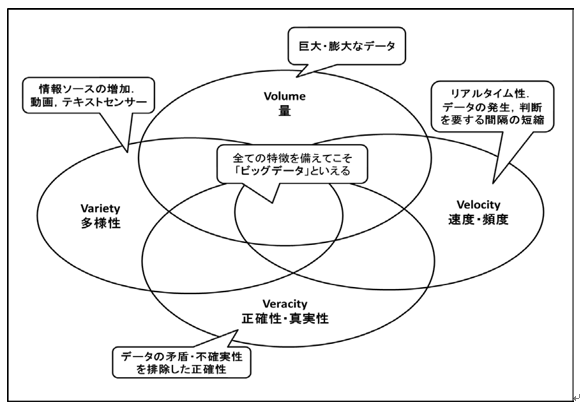
\includegraphics[width=10cm]{bigdata4v.png}
\caption{ビッグデータの4V}\label{サンプル図}
\end{figure}


\section{3Vでのビッグデータの定義}

3Vで表す場合は,容量(Volume),種類(Variety),頻度・スピード(Velocity)の3つになり,正確さ(Veracity)は含まれない.確かにビッグデータには正確でないデータが混在することもあり,例えばTwitterなどのSNSデータには,冗談やデマ情報の書き込みなども混じっており,センサーなどでも故障によるノイズが混じることもあります.データ量が少ない場合には,外れ値として手作業で除去することも可能だがいわゆるビッグデータと言われている大量のデータの場合は,手作業によるデマ情報やノイズなどの除去はほとんどふかのうである.

しかし,ビッグデータで収集するデータは殆どが生データであるという特徴がある.正確さをどう定義するにもよるが,センサーからの入力データなどは生データそのものだが,SNSからの入力データなども生データであり,その意味では正確なデータといえる.つまり,編集などで手が加わっていないデータであり,またそこで発せられるメッセージはその人が,その人の環境により制約などを感じるデータではないからだ.これは,勤務する企業・組織内で作成する報告書などと対比して考えるとわかりやすいだろう.

\section{ビッグデータ処理のパターン}

下記の表に,3つの処理パターンの特性を簡潔にまとめたものを記述する.

\begin{table}[H]
  \begin{tabular}{|l|l|l|l|} \hline
                     & バッチ処理 & インタラクティブクエリー処理 & ストリームデータ処理 \\ \hline
    実行タイミング & ユーザー指定と定期的実行 & ユーザー指定と定期的実行 & 常時連続実行 \\ \hline
    処理単位 & 蓄積データをバッチで一括処理 & 蓄積データをバッチで一括処理 & 少数のフローデータ処理 \\ \hline
    実行時間 & 分~時間 & 秒~分 & ミリ秒~秒 \\ \hline
    処理モデル & MapReduce & クエリ・OLTP & ストリーム処理 \\ \hline
  \end{tabular}
\end{table}


ビッグデータの処理パターンには,「バッチ処理」,「インタラティブクエリー処理」,「ストリームデータ処理」の3種類のパターンがある.

 バッチ処理では筑西データをバッチで一括処理だが,これはGoogle検索用に開発されたMapReduce処理を利用したHadoopが代表的である.しかし,Hadoopはビッグデータ処理用として開発されたものではないので,処理結果作成に時間がかかるという欠点がある.

インタラティブクエリー処理は,蓄積された大容量データをオンラインクエリなど使用して一括解析処理するものである.インタラティブクエリー処理では蓄積されたビッグデータを数秒から数分で実行する.

ストリームデータ処理は大量発生する実世界データを逐次に時系列処理する技術である.データ発生時にあらかじめ登録したシナリオにしたがって集計・分析に必要なデータを抽出し,データ処理を行う.このように逐次時系列でデータ処理できることから,最新の情報,その中での特異な値の発生などに対してリアルタイムに対応するシステムを構築できることが特徴でIoTへの応用に最適な処理方法といえる.\cite{bigquerystart}


\subsection{バッチ処理}

最初にMapReduceで代表される,バッチ処理の特性を見る.

数十年前のメインフレームは,主記憶が数百キロバイト,価格は数千万程度だった.これを現在のPC(主記憶数ギガバイト,価格は10万円程度)と比べた場合,価格性能比では約100万倍にもなる.また,CPU処理スピードと,ネットワークの帯域幅についてはそれぞれ,主記憶と類似の性能向上を遂げてきている.

このようなことは,コンピューター関係以外の業種ではまったく例を見ない群を抜く性能向上である.この急激なプラットホームの真価がクラウドコンピューティングやそのうえで実行されるビッグデータ処理などを可能にしている.\cite{bigquerystart}

ただし,これはクラウドなどに限ったことではない.ITの世界ではこれまでも短いタイムスパンで新しいテクノロジー・ブレークスルーやビジネスモデルが出現してきており,これはプラットホームやネットワークの新派に依存している部分が多くある.言葉を変えれば,これらの新しい発想はその時点でのプラットホーム性能で初めて成り立つものであり,これをわずかでも前の世代に思いついたとしても,実現不可能である場合が多い.

このようにクラウドなどの先端ITシステムは,現在のそしてこれからも進化を続けるはずのプラットホームやネットワークに依存したものである.\cite{bigquerystart}

\subsection{インタラティブクエリー処理}

インタラティブクエリー処理は,BigQueryによる説明を記述する.Googleがリリースするソフトウェアツールには,もともとGoogleが社内使用の目的で開発していたものも多く,BigQueryもそれに当てはまる.Googleも当初は社内使用でもMapReduceを使用してビッグデータ処理を行っていたが,バッチ処理による結果生成の遅延や処理を行うための準備の煩雑さなどから,それに代わるツールとして開発されたのがBigQueryである.
BigQueryはデータの入力はまたはJSONフォーマットのファイルから直接行うことができる.また,Cloud Storageからのデータロードも可能である.ビッグデータの解析や絞込みはRDB(Relational Database)のSQLに類似したクエリ言語を使用し,UI画面やPCのコマンドラインから容易にデータ検索を行うことができる.他にもExcelを使用し検索・表示を行うことが出来る.\cite{bigquerystart}


%図の挿入
\begin{figure}[H]
\centering
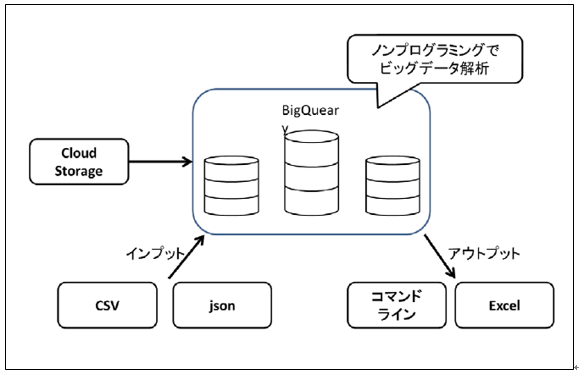
\includegraphics[width=10cm]{bigqueryinout.png}
\caption{BigQueryの入出力}\label{サンプル図}
\end{figure}


BigQueryを使用したインタラクティブクエリ処理では,マウス操作と簡単なキー入力によって全ての操作を行うことができる.また結果出力も数秒から数分以内で得ることができる.したがって,何かこのデータを解析したいと考えたとき,その場で気軽に行えるという点が一番の特徴として挙げられる.

BigQueryでのビッグデータ解析は大量のデータを超高速で行えるのも大きな特徴である.例として,15億行のデータに対する比較的複雑な集計問い合わせが20秒から25秒で返ってきたというユーザの実行結果もある.BigQueryでは,インデスクを作成する必要がなくデータをロードするだけでこのような高速クエリが実行できる.キャッシュは戸鶴ボタンから有効無効を切り替えられるが,キャッシュを使っていなくても,使っているばあ地と同様の結果が得られる.\cite{bigquerystart}


\subsection{ストリームデータ処理}

ストリームデータ処理は,大量発生する時系列のデータ(ストリームデータ)をリアルタイムに逐次処理する技術.

ストリームでたー処理は,データ発生時に,あらかじめ登録したシナリオにしたがって集計・分析に必要なデータを抽出し,データ処理を行う.その際,分析対象データをメモリー上で処理する「インメモリデータ処理技術」により,高速なデータ処理を実現している.これらの技術によって,大量データを高速に,かつリアルタイムに処理できる.例えば,株価のテクニカル指標やランキング情報から売買をリアルタイムに自動判定する.といったシステムに大変有効である.他にも,リアルタイムの在庫管理や,不正操作の監視を行うシステムなど,多くの利用目的が考えられる.\cite{bigquerystart}

%図の挿入
\begin{figure}[H]
\centering
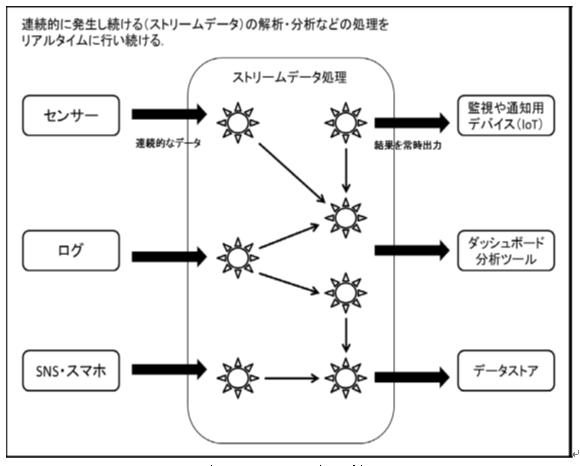
\includegraphics[width=10cm]{streamdatasyori.png}
\caption{ストリームデータ処理}\label{サンプル図}
\end{figure}





\chapter{目的}

研究目的

Wikipediaを一つのプロジェクトとみなし,このオンライン百科事典で品質管理がどのように行われているか調査する.この調査により,オープンな共同作業プロジェクトにおける,品質管理マネジメントのあり方についての知見を得たい.


プロジェクトマネジメントとの関連

本研究は,プロジェクトマネジメントを学ぶことを目的としているため,プロジェクトマネジメントとの関連が全面的にある.

考案するゲームは,プロジェクトマネジメント知識体系ガイド(PMBOK@ガイド)の第4版(以下,PMBOK)を参考にし,プロジェクトマネジメントとの一連の活動や,PMBOKに記載されている9つの知識
エリアについての内容を活用する.\cite{PMBOK}

PMBOKとは,プロジェクトマネジメントに関する知識体系である.

現在は,PMBOKに従ってプロジェクトマネジメントを実施することが,デファクトスタンダードになっている.

PMBOKに記載されている9つの知識エリアとは,何をやるべきかという観点,何を管理するべきかという観点からみたものである.

9つの知識エリアは,以下9つのマネジメントについての内容となっている.


\begin{enumerate}
 \item プロジェクト統合マネジメント
 \item プロジェクト・スコープ・マネジメント
 \item プロジェクト・タイム・マネジメント
 \item プロジェクト・コスト・マネジメント
 \item プロジェクト品質マネジメント
 \item プロジェクト人的資源マネジメント
 \item プロジェクト・コミュニケーション・マネジメント
 \item プロジェクト・リスク・マネジメント
 \item プロジェクト調達マネジメント
\end{enumerate}








本研究では,上記のPMBOKの中の品質マネジメントが関連性が最もあるものであるといえる.このオープンなプロジェクトの百科事典は記事の作成や,編集が主に行われて創り上げられており,その成果物がこの百科事典である.


成果物のイメージ
 差し戻しに関するデータを収集し,編集回数や頻度などの要素を洗い出す.そして,いくつかの要素から条件を決めクラスター分析を行う.その結果から悪意のある編集がされている記事に共通する点を見つけ,Wikipediaのオープンなプロジェクトでの品質マネジメントの知見を得る.




\chapter{手法}

研究方法

\begin{enumerate}
 \item Wikipedia日本語版の編集履歴まで含んだファイルをダウンロードし,ローカルでデータマイニングを行う.
 \item Wikipediaの管理者の編集回数の変化を解析する.
 \item 管理者の編集の割合がプロジェクトの動きにどのようにつながっているのか調査する.
\end{enumerate}

研究を行うための用意

開発環境としてLinuxを扱う.そのために,VirtualBoxとubuntuを用意する. またプログラミング言語はpythonを使用した.



\section{VirtualBoxとは}

使用しているパソコン上に仮想的なパソコンを作成し,別のOSをインストール・実行できるフリーのパソコン仮想化ソフトのことである.本研究では,LinuxOSを扱いたいが,パソコン本体はWindowsOSの為,このソフトを利用する.


%図の挿入
\begin{figure}[H]
\centering
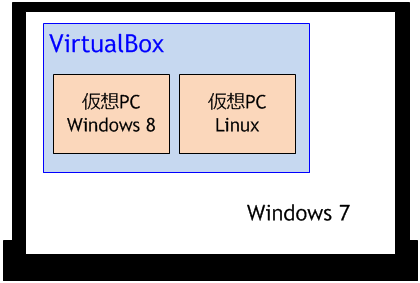
\includegraphics[width=10cm]{sample10.png}
\caption{図の挿入例}\label{サンプル図}
\end{figure}





VirtualBoxはコンピュータ上で直接動作している通常のOSにとってはアプリケーションの一つであり,他のソフトと同じように起動することができる.起動すると仮想的なコンピューターが構築され,元のOSとは独立に別のOSを起動することができる.VirtualBoxが実行されているOSをホストOS,VirtualBox上で実行されているOSをゲストOSという.

元は独立系のソフトウェア企業が開発・販売していた製品だった.しかし,開発元がSun Microsystems社に買収され,その後同社がOracle社に買収されたため,Oracle社が開発元となり,正式名称も「Oracle VM VirtualBox」となった.また,VirtualBox本体はGPLに基づいたオープンソースソフトウェアとして公開され,誰でも自由に入手・利用・改変・再配布などが行える.

VirtualBoxを使う上での注意点

現時点でのVirtualBoxは仮想メモリをサポートしていないため,実メモリ以上のメモリを仮想PCが使用することはできない.仮想メモリを使うと動作が遅くなるため,仮想PCには実メモリ以内のサイズを割り当てる.そのため,仮想PCを1台だけ起動するのであれば問題ないが,複数の仮想PCを同時に起動させる場合これがネックになってしまう.同時起動させる全ての仮想PCのメモリサイズの合計が実メモリのサイズを超えないようにする.そのため,VurtualBoxをインストールするPCには多くのメモリが必要で,最低4GB以上のPCを使うようにするべきである.


%次のページに移動
\clearpage


\section{VirtualBoxのインストール}

\subsection{ダウンロード}

Oracleが提供しているOracleVirtualBoxというのを下記のサイトからダウンロードする.本研究ではWindowsOSを使用しているので,VirtualBox platform packagesの中にある「VirtualBox 5.0.4 for Windows hosts」 というのを選択する.

%図の挿入
\begin{figure}[H]
\centering
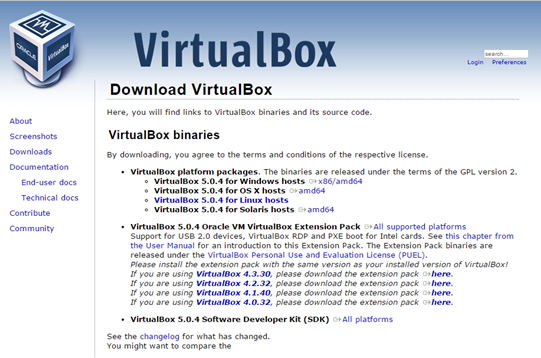
\includegraphics[width=13cm]{VirtualBox.png}
\caption{ダウンロードサイト}\label{サンプル図}
\end{figure}


ダウンロードサイト

https://www.virtualbox.org/wiki/Downloads


\subsection{インストーラーの実行}

%図の挿入
\begin{figure}[H]
\centering
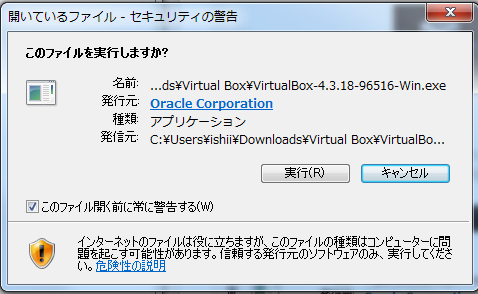
\includegraphics[width=13cm]{VBcaveat.png}
\caption{警告画面}\label{サンプル図}
\end{figure}

インストーラーを起動し,セットアップウィザードを起動する.
「セキュリティの警告」ダイアログが表示された場合は,「実行」をクリックする.


%図の挿入
\begin{figure}[H]
\centering
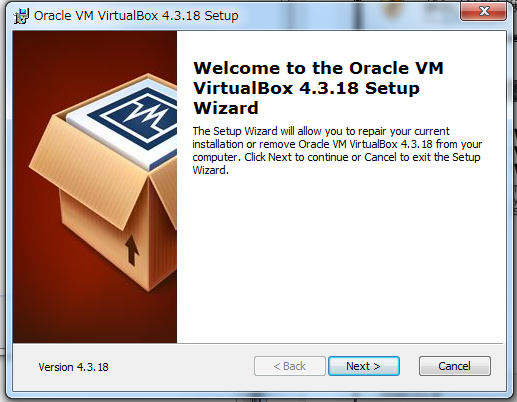
\includegraphics[width=13cm]{VBsetup.png}
\caption{セットアップ画面1}\label{サンプル図}
\end{figure}

右下の「Next」をクリックする.


%図の挿入
\begin{figure}[H]
\centering
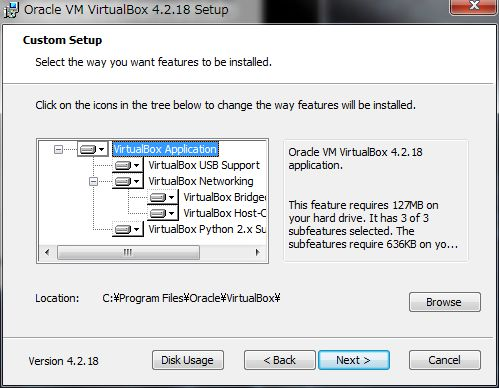
\includegraphics[width=13cm]{VBsetup2.jpg}
\caption{セットアップ画面2}\label{サンプル図}
\end{figure}

VitualBox Applicationを選択したまま,「Next」をクリックする.


%図の挿入
\begin{figure}[H]
\centering
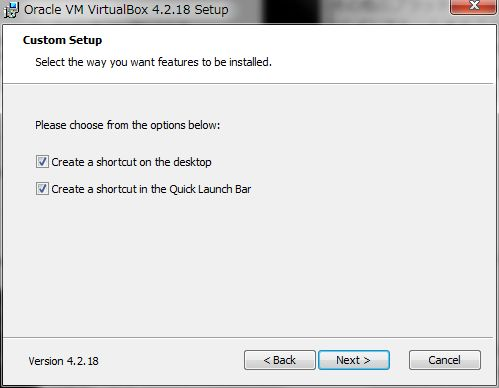
\includegraphics[width=13cm]{VBsetup3.jpg}
\caption{セットアップ画面3}\label{サンプル図}
\end{figure}

2つともチェックマークをつけたまま,「Next」をクリックする.


%図の挿入
\begin{figure}[H]
\centering
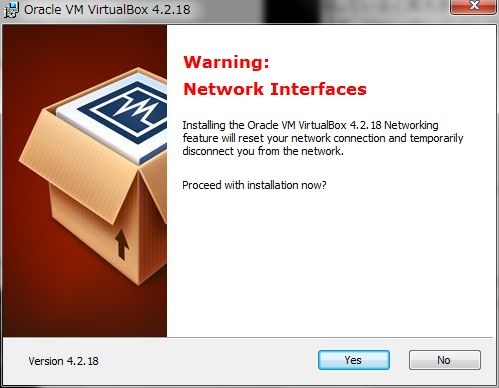
\includegraphics[width=13cm]{Warning.jpg}
\caption{セットアップ画面4}\label{サンプル図}
\end{figure}

Warning:Network Interfaces画面が表示されたら,「Yes」をクリックする.

%図の挿入
\begin{figure}[H]
\centering
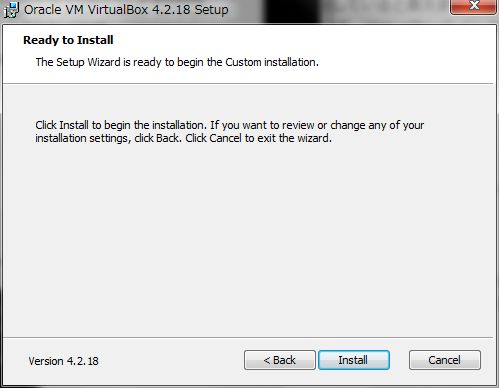
\includegraphics[width=13cm]{Install.jpg}
\caption{セットアップ画面5}\label{サンプル図}
\end{figure}

Ready to Install画面が表示されたら,「Install」をクリックする.

%図の挿入
\begin{figure}[H]
\centering
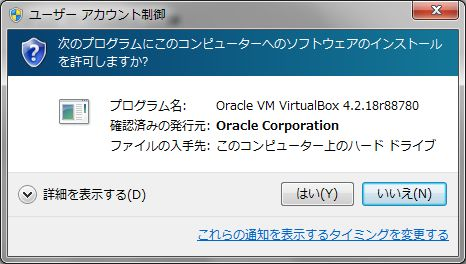
\includegraphics[width=13cm]{useracount.jpg}
\caption{ユーザーアカウント制御画面}\label{サンプル図}
\end{figure}

インストール中にユーザーアカウント制御によって,ソフトウェアのインストールを許可する必要がある.

その場合は画面が表示されるので,「はい」をクリックする.


%図の挿入
\begin{figure}[H]
\centering
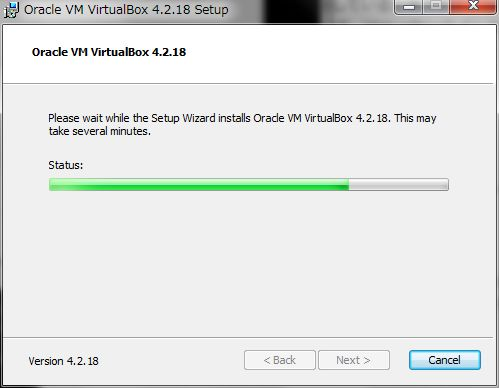
\includegraphics[width=13cm]{It_is_install.jpg}
\caption{インストール中の画面}\label{サンプル図}
\end{figure}

インストール実行画面になるので、終了するまでそのままにする.

%図の挿入
\begin{figure}[H]
\centering
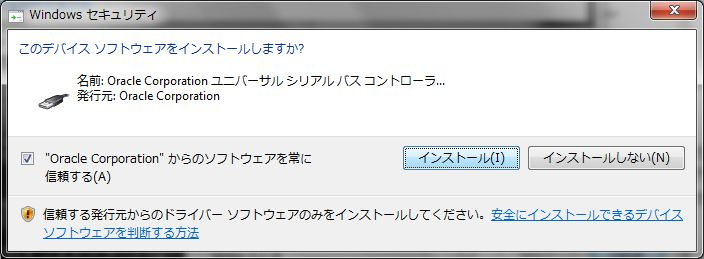
\includegraphics[width=13cm]{device_install.jpg}
\caption{Windowsセキュリティの画面}\label{サンプル図}
\end{figure}

Windowsセキュリティの画面が表示されたら,「'OracleCorporation'からのソフトウェアを常に信頼する」というところにチェックし,インストールをクリックする.

%図の挿入
\begin{figure}[H]
\centering
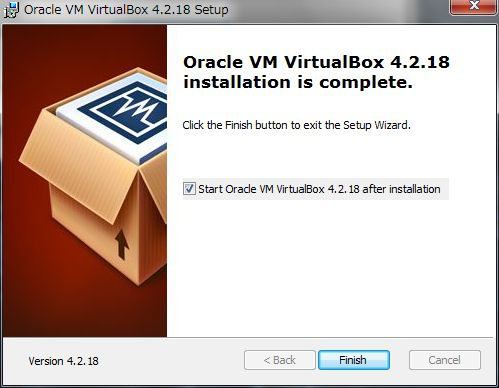
\includegraphics[width=13cm]{install_finish.jpg}
\caption{インストール完了の画面}\label{サンプル図}
\end{figure}

インストールが完了すると,インストール後にVirtualBoxを起動するか聞かれる.起動してもしなくても構わない.

「Finish」をクリックすれば,インストール完了.


%図の挿入
\begin{figure}[H]
\centering
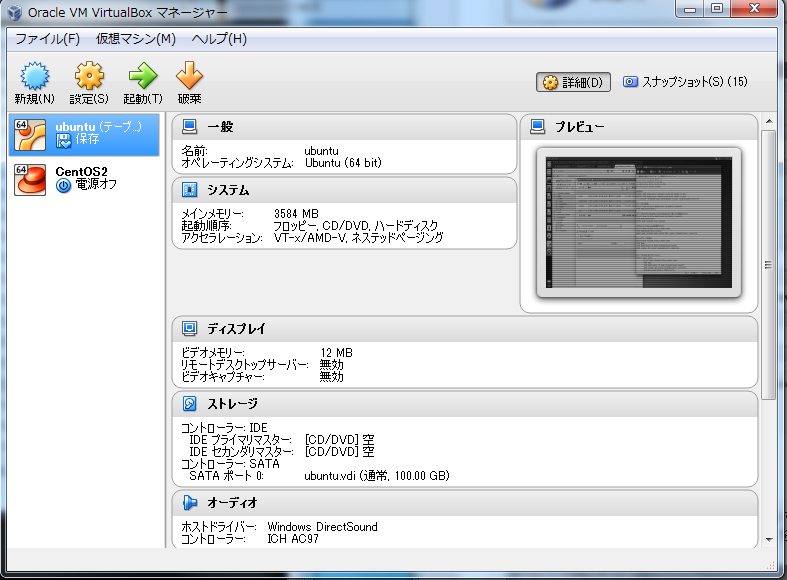
\includegraphics[width=13cm]{VirtualBox_start.png}
\caption{VirtualBox起動時の画面}\label{サンプル図}
\end{figure}

インストールした「VirtualBox.exe」を起動して正常に動くか確認する.






\section{用語}

本節では,本研究で利用するVirtuaklBoxの用語について説明する.


\subsection{ホストマシン(物理マシン)}

物理的に存在するコンピュータのこと.

\subsection{ホストOS}

ホストマシンにインストールされているOSのこと.VirtualBoxはホストOSにインストールされる.

\subsection{バーチャルマシン(仮想マシン)}

VirtualBoxが作成する論理的なマシンのこと.ゲストマシンに割り当てるために,VirtualBoxがホストマシンのコンピュータ資源(CPUやメモリ,HDD等)の一部を仮想化する.ホストマシンの資源を使いきらない限り,ゲストマシンを複数作成したり,多重起動させることができる.

\subsection{ゲストOS(仮想OS)}

ゲストマシンにインストールされるOSのこと.本研究では,Ubuntuというものをインストールする.

\subsection{仮想ディスク}

ゲストマシンが使用する仮想のハードディスクのこと.バーチャルマシンからはこれを物理ディスクとして扱うことができる.仮想ディスクの実態はホストマシン内にファイルとして存在する.



\section{Ubuntuとは}

Ubuntu(ウブントゥ)とは,コミュニティにより開発されているオペレーティングシステムのこと.ラップトップ,デスクトップ,そしてサーバーに利用することができる.Ubuntuには,家庭・学校・職場で必要とされるワープロやメールソフトから,サーバーソフトウェアやプログラミングツールまで,あらゆるソフトウェアが含まれています.

Ubuntuは現在、そして将来に渡って無償で提供されます。ライセンス料を支払う必要はありません。Ubuntuをダウンロードすれば、友達や家族と、あるいは学校やビジネスに、完全に無料で利用できます。

提供会社は,新しいデスクトップおよびサーバーを6ヶ月ごとにリリースすることを宣言している。これにより、オープンソースの世界が提供する最新の優れたアプリケーションを常に利用できる。


%次のページに移動
\clearpage

\section{Ubuntuのインストール}

\subsection{ISOイメージをダウンロードする}

まず,https://www.ubuntulinux.jp/download/ja-remix よりUbuntu 14.04 のISO イメージをダウンロードする.本研究では64bit 版を選択した.



%図の挿入
\begin{figure}[H]
\centering
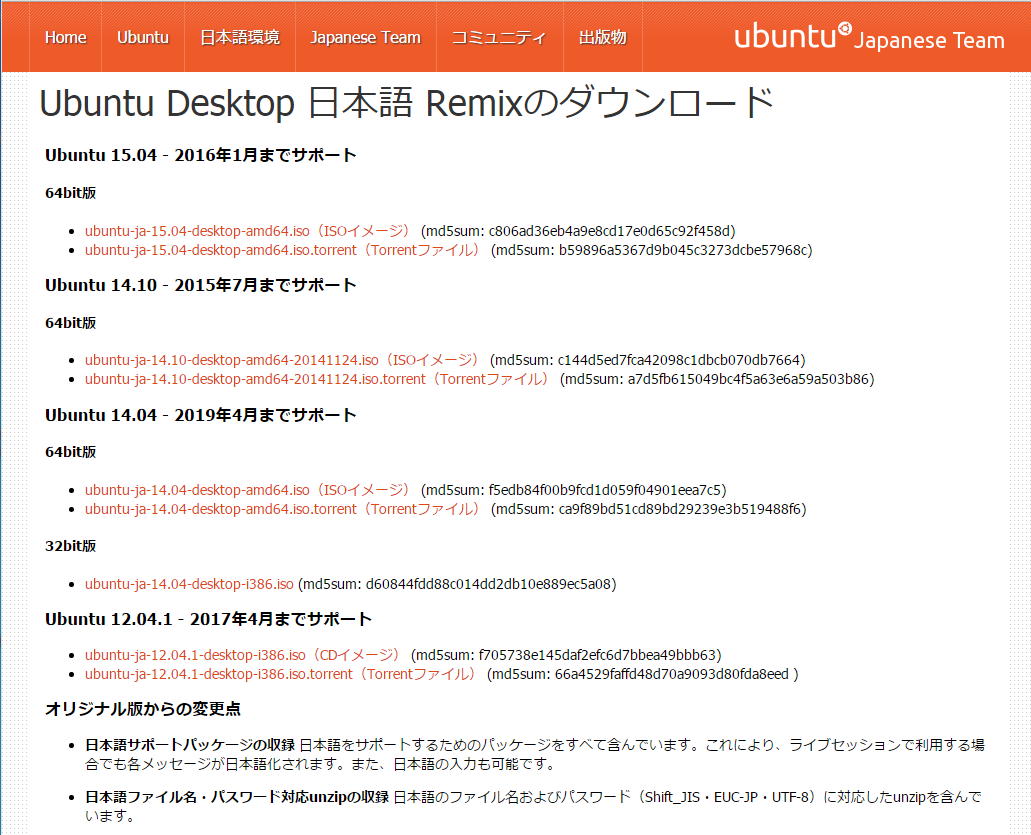
\includegraphics[width=10cm]{UbuntuDL.png}
\caption{UbuntuのISOイメージダウンロードページ}\label{サンプル図}
\end{figure}





\subsection{インストールを開始する}

次にインストールしたVirtualBox を立ち上げ,ウインドウ左上にある「新規(N)」のボタンを押してゲストマシンの作成を行う.ゲストマシンの名前,メモリサイズ,HDD の設定をするとウィンドウが閉じられる.

%図の挿入
\begin{figure}[H]
\centering
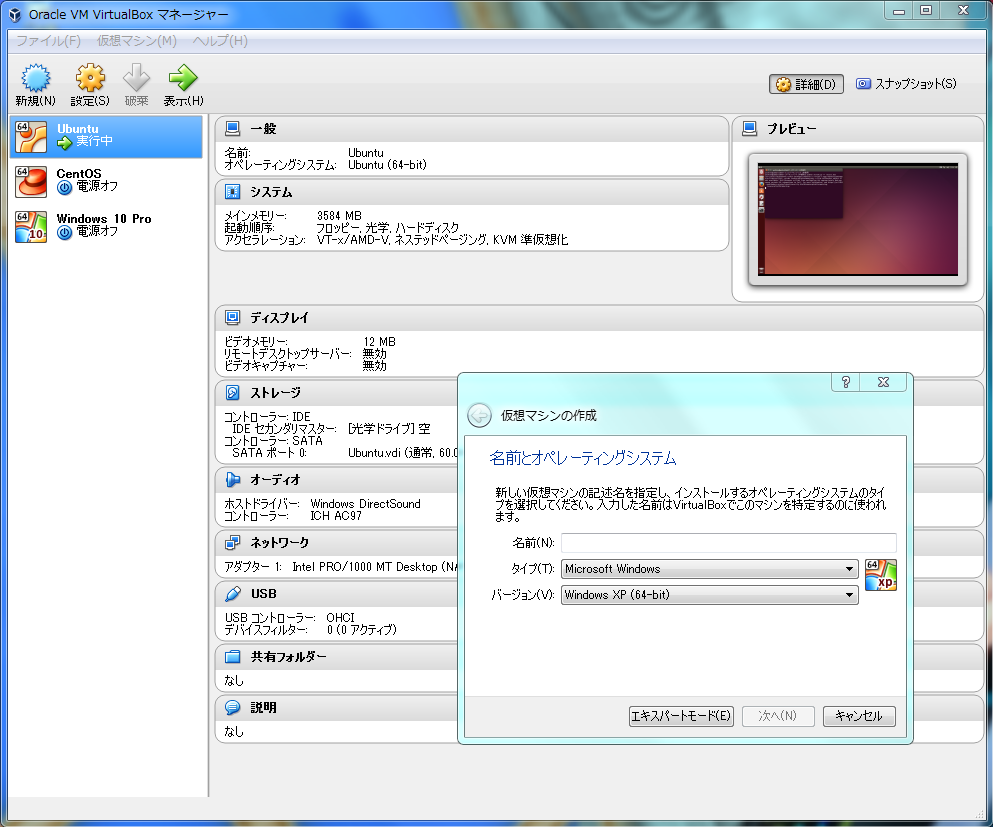
\includegraphics[width=12cm]{VBoxWindow.PNG}
\caption{VirtualBox のウィンドウとゲストマシン作成ウィンドウ}\label{サンプル図}
\end{figure}

続いて「設定(S)」を開き,「ストレージ」の項目からダウンロードしたISO ファイルをセットして「OK」をクリックする.

「起動(T)」を押すとゲストマシンが起動し,Ubuntu のインストールウィザードが表示される.

表示内容に従ってウィザードを進めていくと,ゲストマシン内にUbuntu がインストールされる.


%図の挿入
\begin{figure}[H]
\centering
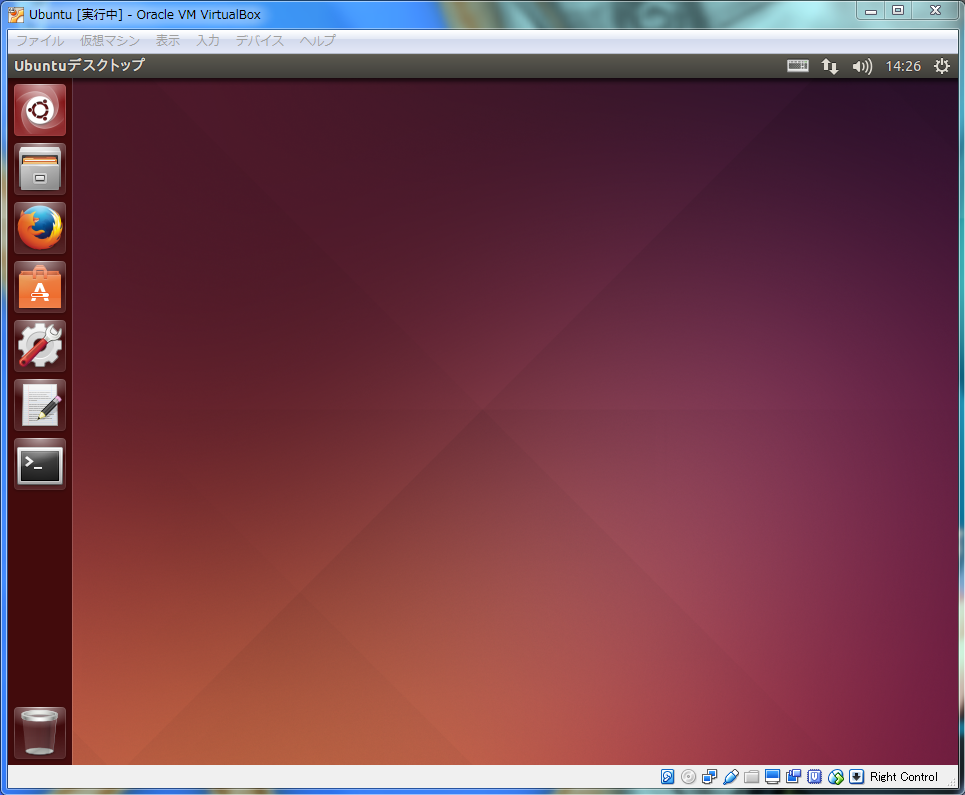
\includegraphics[width=14cm]{Ubuntu_on_VirtualBox.PNG}
\caption{VirtualBox 上で動作するUbuntu}\label{サンプル図}
\end{figure}


\section{端末}

本研究では,ダウンロードしたファイルをUbuntuの端末内で扱う.

起動方法はいろいろあるが,2つ記載する
\begin{enumerate}
 \item ショートカットキーで起動する.

ubuntuの画面を開いた状態で「Ctrl+Alt+T」を押す.このショートカットキーを押すだけで,端末が開く.

 \item コンピュータとオンラインソースを検索」から起動する

Launcherにある「Ubunutuソフトウェアセンター」を開く.「インストール済み」を選択する.
検索ワード欄に「端末」または「ta」と入力する.カテゴリの中に「端末(gnome-terminal)」があるので、それを選択する.

\end{enumerate}


%図の挿入
\begin{figure}[H]
\centering
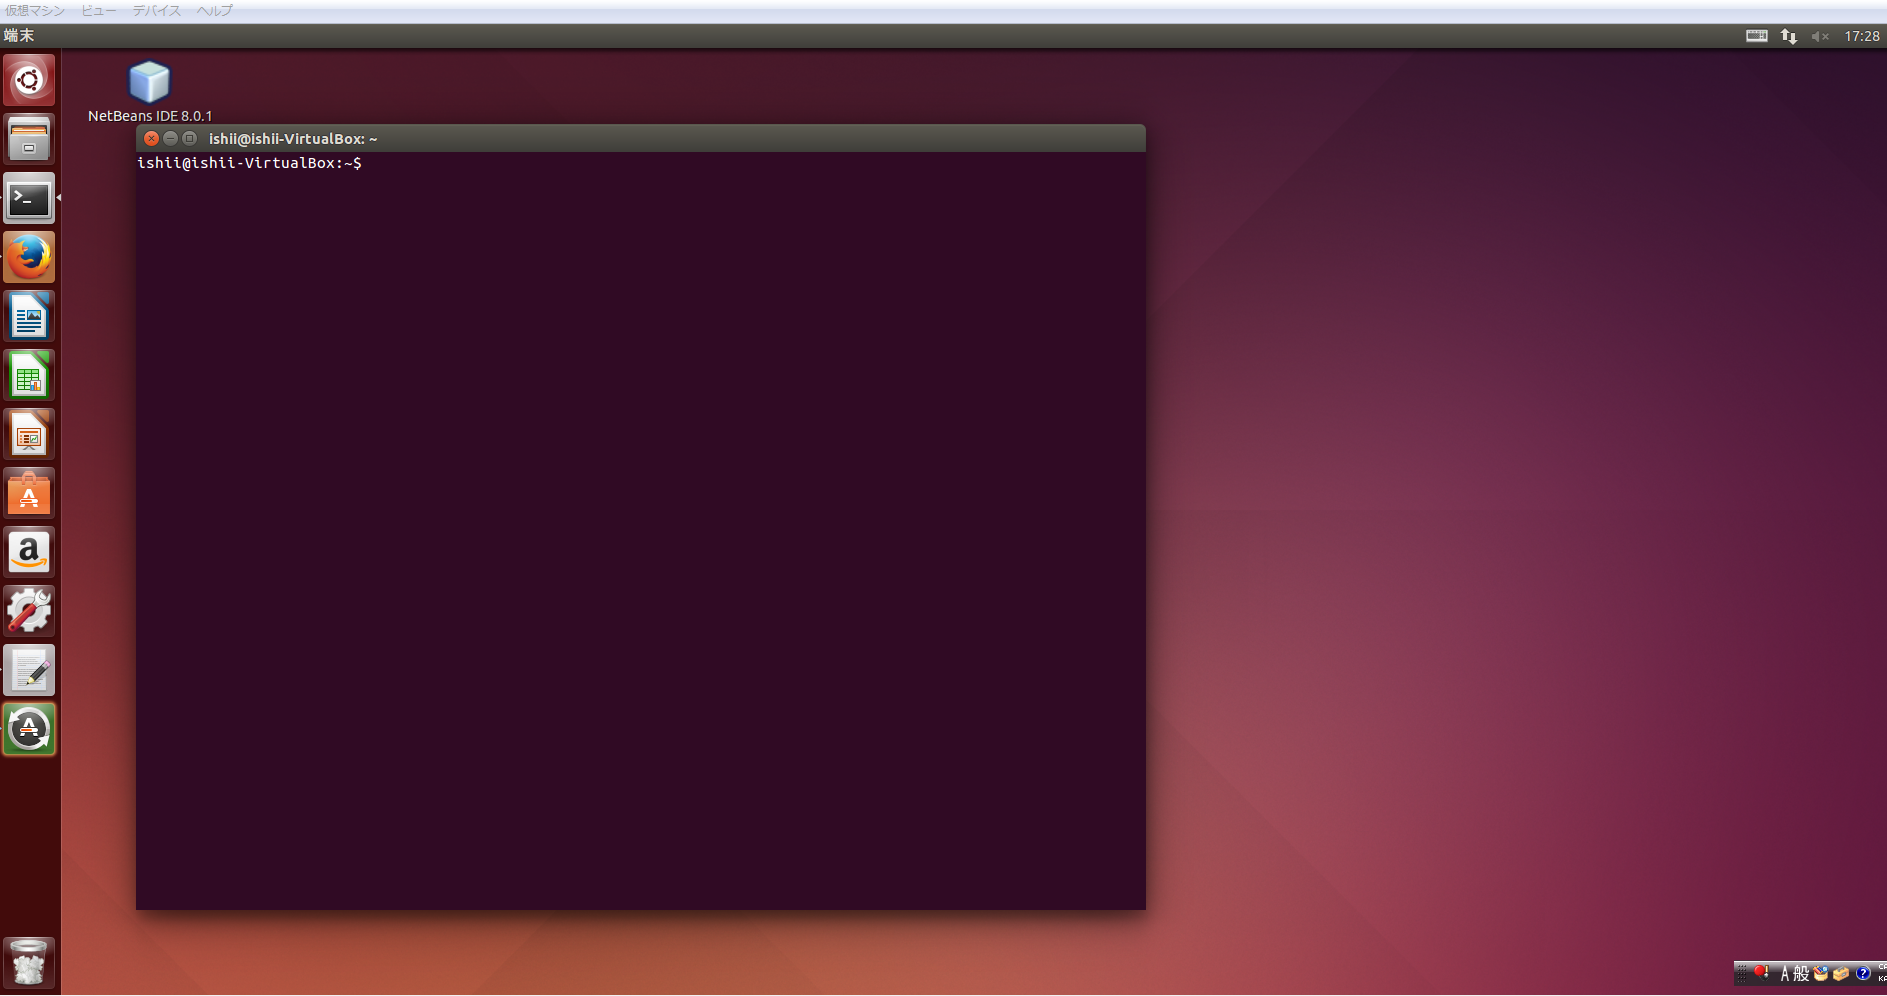
\includegraphics[width=10cm]{tan.png}
\caption{端末を起動した画面}\label{サンプル図}
\end{figure}



\section{MySQL}

MySQLの操作,そこで使用したSQL文の説明を行う.MySQLの操作は,Ubuntuの端末内とphpmyadmiinで行う.

\subsection{MySQLへのインストール}

Ubuntuでは,以下のコマンドでMySQLをインストールを行う.途中でパスワードを聞かれたら,「pass」のような簡単なものを設定する. \\
{\small
\begin{verbatim}
mysql>sudo apt-get install mysql-server mysql-client
\end{verbatim}}


\subsection{MySQLへの接続}

端末から接続を行う.端末内で次のように入力すればMySQLに接続できる.

mysql -uユーザ名 -pパスワード --default-charcter-set=文字コード

本研究では,ユーザ名は「root」,パスワードは「yasu0705」を入力する.またデータのインポートする際にLOAD文を使いたいので,MySQLの接続時に「mysql --local-infile・・・」と入力する.

以下のように接続を行う. 

{\small
\begin{verbatim}
mysql>mysql -uroot -pyasu0705 --local-infile --default-character-set=utf8
\end{verbatim}}

%図の挿入
\begin{figure}[H]
\centering
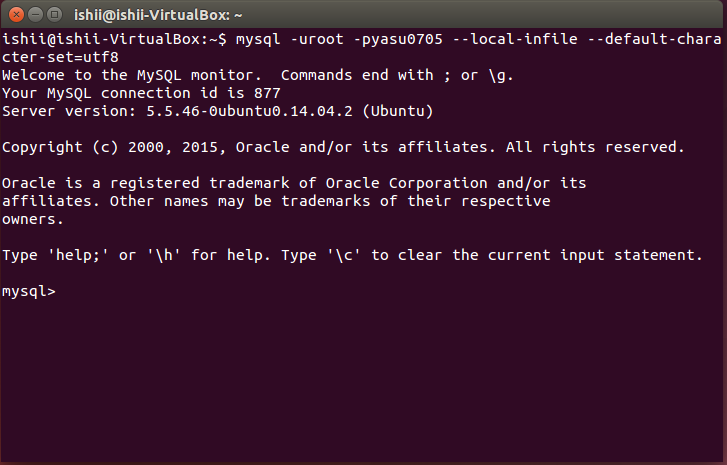
\includegraphics[width=10cm]{MySQL_connection.png}
\caption{MySLQ接続画面}\label{サンプル図}
\end{figure}

\subsection{phpmyadmin}

PHPで実装されたMySQLの管理ツール.MySQLのデータベースやテーブルの作成を行ったり,データの追加や参照などを作成することなくブラウザから行うことができる.

%図の挿入
\begin{figure}[H]
\centering
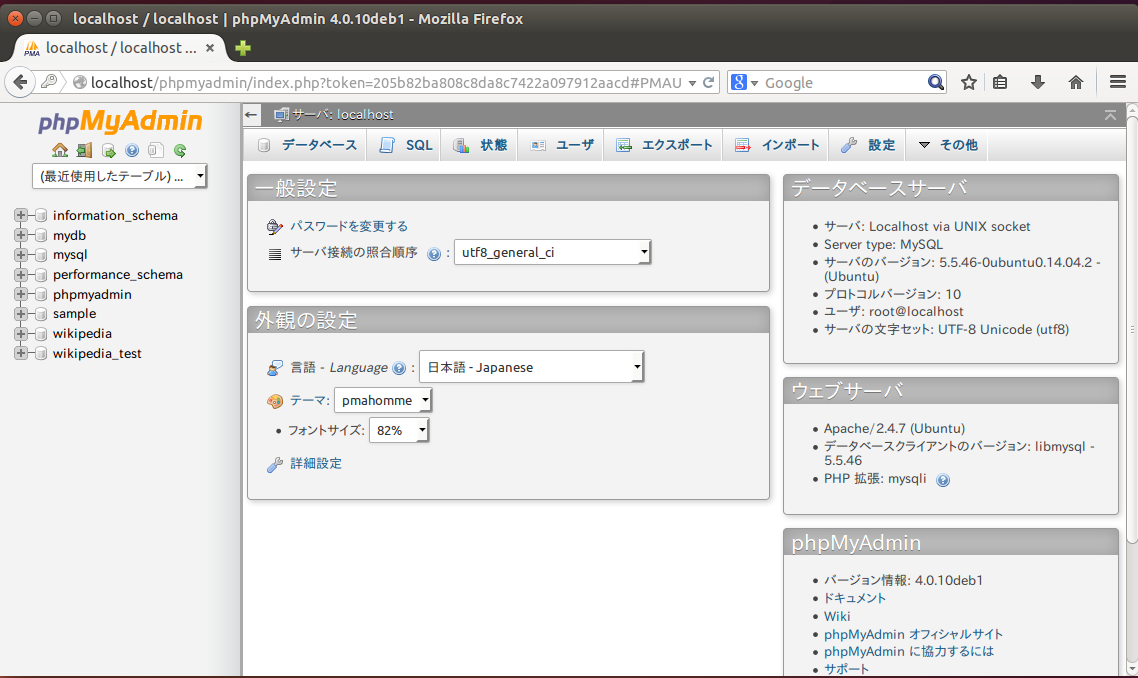
\includegraphics[width=10cm]{phpmyadmin_main.png}
\caption{phpmyadminのメインページ}\label{サンプル図}
\end{figure}

%次のページに移動
\clearpage


\section{Wikipediaの編集履歴データの取得}

\subsection{ファイルのダウンロード}

日本語版Wikipediaのデータは,https://dumps.wikimedia.org/jawiki/からダウンロードできる.

%図の挿入
\begin{figure}[H]
\centering
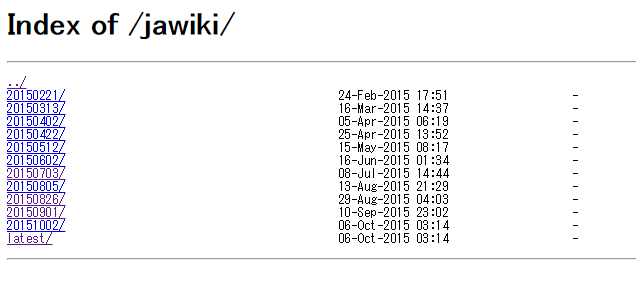
\includegraphics[width=14cm]{Index_of_jawiki.PNG}
\caption{日本語版Wikipediaデータダウンロードサイト}\label{サンプル図}
\end{figure}

再現性を確保するため,20150901番を扱う.latestだと,最新だが,日々更新されて変更されてしまう可能性があるため今回は利用しない.



データの中身にどのようなものが調べた.\cite{wikipedia_data_list}調べた結果,stub-meta-history.xmlが使えそうなので,これを利用する.また、「stub-meta-history1」などの分割ファイルも利用する.

%図の挿入
\begin{figure}[H]
\centering
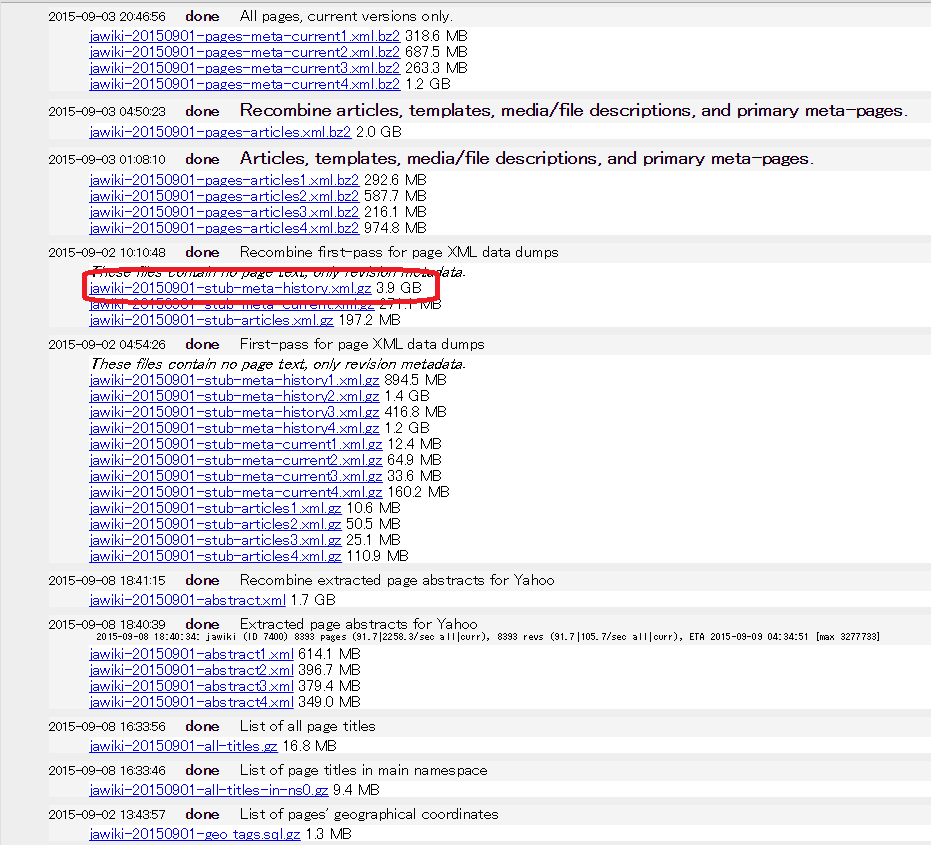
\includegraphics[width=14cm]{wiki20150901.PNG}
\caption{20150901のstub-meta-history}\label{サンプル図}
\end{figure}



\section{XMLファイル}

WikipediaのデータはXMLというものだった.XMLとは,ExtensibleMarkupLanguageの略であり,インターネット上でさまざまなデータを扱う倍いに利点があるファイルである.1998年にでた比較的新しい言語だが,仕様が簡単なため,広く使用されるようになった.

XML文書はテキストファイルの形で存在するため,そのままソフトで利用することが出来ない.個々のソフトの中にXML文書を解釈するプログラムを持たせる方法があるが,XMLは一定の形式が定められているため,汎用的な解釈プログラムであるXMLパーサーによって変換したデータをソフトが使うようにした方が効率が良い.アプリケーションソフトでXML文書を扱う場合には,直接XML文書を読むのではなく,XMLパーサを扱うのが一般的になっている.\cite{xml1}




\section{XMLパーサ}

XML文書を,アプリケーションソフトが利用しやすい形に変換するソフトウェアのこと.変換時に,XML文書が文法に照らして性格に記述されているかどうかを同時に検証するものである.

XMLパーサの中にはDOM(Document Object Model)と,SAX(Simple API for XML)という最も広く利用されている標準的なAPIがある.

本研究では,このXMLの文書の操作には.SAXパーサというものを用いて扱う.Wikipediaの編集履歴データは膨大な為,木構造として全てのデータを読み込んでから処理するDOMパーサでは,データの扱いが困難なためである.



\subsection{DOMパーサ}

DOMとは,XML文書やHTML文書を構成する要素をコンピュータプログラムで参照したり操作したりするための取り決め(API)の1つである.

HTMLやXMLで記述されたWebページなどの構成要素(見出し,段落,領域,画像,リンクなど)と,それらの配置は見栄えなどを定めた属性情報などを参照,制御する手法を定めている.Webブラウザなどに実装されており,ページ上にJavaScriptなどで記述されたスクリプトからページ内の各要素を読み取ったり,内容や設定の変更,要素の追加や削除などを行う標準的な手段として用いられる.

文書をDOMで表したデータは,文書の最上位の要素を頂点として,各要素が枝分かれしていく木構造(ツリー構造)となっており,これを「DOMツリー」と呼ぶこともある.\cite{DOM1}



\subsection{SAXパーサ}

XML文書の解釈や検証を行う「XMLパーサー」というプログラムを利用する際に使う利用手順の1つである.また,DOMと並んで最も広く利用されているAPIの1つとして使われる.

XML文書を一つの木構造に変換するDOMと違って,XML文書を先頭から一行ずつ読み込んで,要素が現れるたびに対応する処理手順を呼び出すという方式を用いている.よって巨大なXMを扱ってもメモリに負担がかからず高速に処理できるという特徴がある.その反面,文書の構造を自由にたどれないので,処理の柔軟性に劣り,複雑な処理には向かない.\cite{SAX1}



\section{pythonとは}

広く使用されている汎用のプログラミング言語の1つである.コードの読み取れる性質が高くなるように言語が設定されている.その構文のおかげで,Cなどの言語と比べると,より少ないコード行数でプログラムを表現できる.小規模なプログラムから大規模なプログラムまで,さまざまなプログラムをクリアに書けるように,多くのコードが提供されている.

\subsection{インストール方法}

当研究では,ubuntuで行うので,以下のコマンドを端末で入力すればインストールできる.

{\small
\begin{verbatim}

sudo apt-get install pythonバージョン

例えばバージョン2.7をインストールしたい場合は以下のようにすればよい.

sudo apt-get install python2.7
\end{verbatim}}


\subsection{バージョンの確認}

以下のコマンドで,バージョンの確認ができる.


{\small
\begin{verbatim}
python --version
\end{verbatim}}




\chapter{結果}



\section{Wikipediaの履歴の調査}



ダウンロードしたファイルの中身がどんななのか確認するため,以下のコマンドを入力する.qボタンを押すと終了する.
{\small
\begin{verbatim}
gunzip -c jawiki-20150901-stub-meta-history.xml.gz | less
\end{verbatim}}

%図の挿入
\begin{figure}[H]
\centering
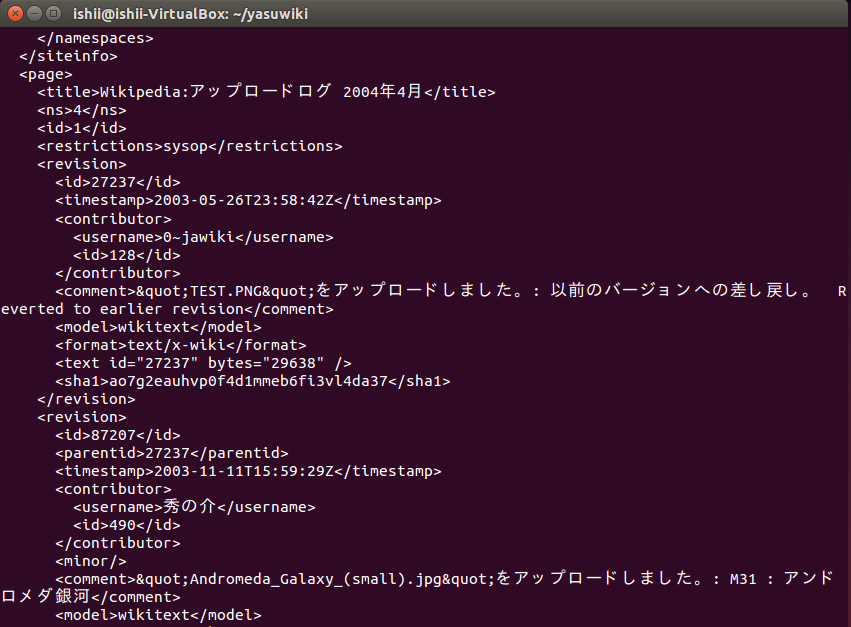
\includegraphics[width=12cm]{jawiki_contents.png}
\caption{lessで中身確認}\label{サンプル図}
\end{figure}


\subsection{展開}

展開する際は,「-k」をつける.wikipediaのダウンロードファイルは時間がかかるため,一度ダウンロードしたら消さずに取っておく.

{\small
\begin{verbatim}
gunzip -k jawiki-20150901-stub-meta-history.xml.gz

gunzip -k jawiki-20150901-stub-meta-history{1,2,3,4}.xml.gz
\end{verbatim}}



\subsection{revision数}

ページごとのrevision数を求める.詳細は以下のrevisions.pyを参照. \\
\\
revisions.py

{\small
\begin{verbatim}

# -*- coding: utf-8 -*-

import xml.sax
import sys

class myHandler(xml.sax.ContentHandler):
  reading = {"title":False}
  title = ""
  revisions = 0

  def __init__(self):
    xml.sax.ContentHandler.__init__(self)
 
  def startElement(self, name, attrs):
    self.reading[name] = True
 
  def endElement(self, name):
    self.reading[name] = False
    if name == "page":
      print(self.title + "\t" + str(self.revisions))
      self.title = ""
      self.revisions = 0
    elif name == "revision":
      self.revisions = self.revisions + 1
 
  def characters(self, content):
    if self.reading["title"] == True:
      self.title = self.title + content
  
def main():
  xml.sax.parse(sys.stdin, myHandler())
 
if __name__ == "__main__":
  main()

\end{verbatim}}





以下のコマンドを入力する. \\

{\small
\begin{verbatim}
cat jawiki-20150901-stub-meta-history.xml | python3 revisions.py | less
\end{verbatim}}


%図の挿入
\begin{figure}[H]
\centering
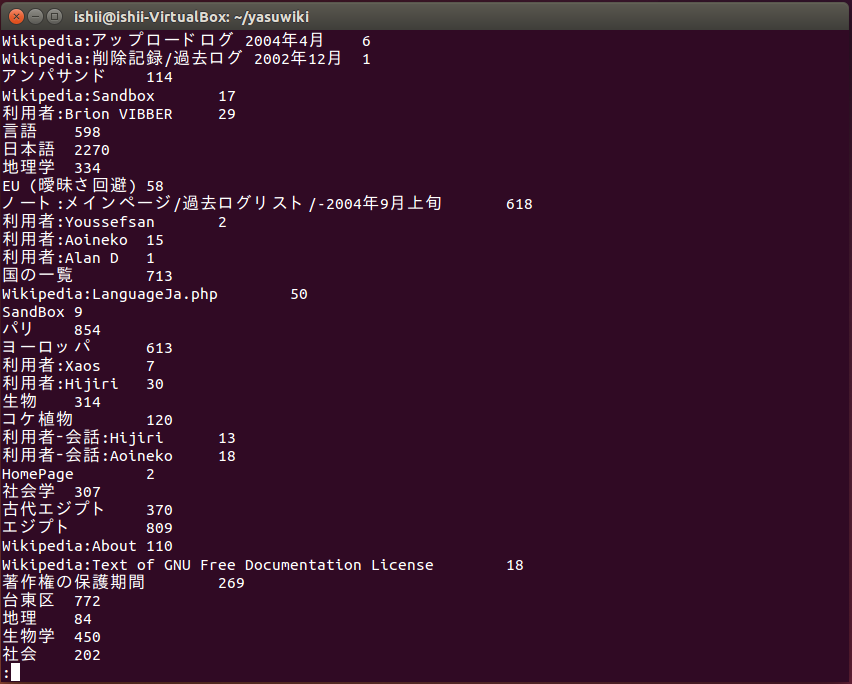
\includegraphics[width=14cm]{wiki_revisions.png}
\caption{revisions数の確認}\label{サンプル図}
\end{figure}

データを取る際は「| less」の部分を「> ファイル名」にする.本研究では,以下のように取得した.

{\small
\begin{verbatim}
cat jawiki-20150901-stub-meta-history.xml | python3 revisions.py > revisions.dat
\end{verbatim}}




次に取得したデータから,revision数が多いページを見つける.詳細は以下のrevisions.shを参照. \\

{\small
\begin{verbatim}
revisions.sh

cat revisions.dat | sort -r -n -k 2 -t "	 " > sort.dat (""の中はTAB)
\end{verbatim}}

以下のコマンドを入力する.

{\small
\begin{verbatim}
time sh revisions.sh
\end{verbatim}}


抽出したデータを確認する為,以下のコマンドを入力する.

{\small
\begin{verbatim}
head sort.dat
\end{verbatim}}


結果は以下のとおり

%図の挿入
\begin{figure}[H]
\centering
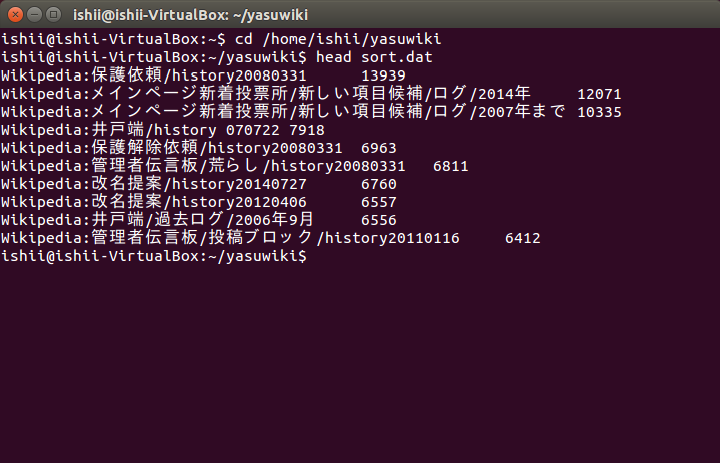
\includegraphics[width=14cm]{head_sort.png}
\caption{revisions数の多いページ}\label{サンプル図}
\end{figure}




\subsection{並列化}

wikipediaの編集履歴データには,「jawiki-20150901-stub-meta-history1.xml」などの分割ファイルがある.これらを扱うことを行う.

準備として,以下のコマンドを入力し,page要素の途中では分割されていないことを確認する.「stub-meta-history」の分割ファイルは4つあるので,4つとも確認する.

{\small
\begin{verbatim}
tail jawiki-20150901-stub-meta-history1.xml

tail jawiki-20150901-stub-meta-history2.xml

tail jawiki-20150901-stub-meta-history3.xml

tail jawiki-20150901-stub-meta-history4.xml
\end{verbatim}}



ファイルの並列化をして,revision数を求める.以下のコマンドを入力する.

{\small
\begin{verbatim}
cat jawiki-20150901-stub-meta-history1.xml | python3 revisions.py > revisions1.dat \&
cat jawiki-20150901-stub-meta-history2.xml | python3 revisions.py > revisions2.dat \&
cat jawiki-20150901-stub-meta-history3.xml | python3 revisions.py > revisions3.dat \&
cat jawiki-20150901-stub-meta-history4.xml | python3 revisions.py > revisions4.dat \&
\end{verbatim}}

次に結合してソートするため,以下のコマンドを入力する.

{\small
\begin{verbatim}
cat revisions{1,2,3,4}.dat | sort -r -n -k 2 -t "   " > sort-parallel.dat
\end{verbatim}}

データを抽出したら「head sort-parllel.dat」で結果を確認する. \\
「diff sort.dat sort-parallel.dat」で,一括データと分割データの違いを見る.結果が空,つまり両者に違いが無ければ同じデータが取れている.

%次のページに移動
\clearpage


\subsection{差し戻し回数}

「stub-meta-history」のデータの中には,SHA1が入っていた.SHA1とは,認証やデジタル署名などに使われるハッシュ関数のひとつである.2の62条ビット以下の原文から
160ビットの「ハッシュ値」を生成し,通信経路の両端で比較することで,通信途中で原文が改ざんされていないかを検出することが出来る.

このSHA1が同じなら差し戻しとみなすことにする.ただし,以下の問題はある.
\begin{itemize}
 \item テキストが違ってもSHA1が同じになることはある.
 \item 差し戻してそのまま編集された場合をかうんとできない.
\end{itemize}

SHA1を単純にか添えた結果が編集回数にする.そこから重複を削除した結果が差し戻し以外の回数とし,両方の差が,ここでいう差し戻しの解すという定義にする.
詳細は以下のrevert.pyを参照.\\
\\
revert.py

{\small
\begin{verbatim}

# -*- coding: utf-8 -*-

import xml.sax
import sys

class myHandler(xml.sax.ContentHandler):
  reading = {"title":False, "sha1":False}
  title = ""
  revisions = 0
  sha1 = ""
  sha1s = set() #SHA1を数える(重複なし)

  def __init__(self):
    xml.sax.ContentHandler.__init__(self)
 
  def startElement(self, name, attrs):
    self.reading[name] = True
 
  def endElement(self, name):
    self.reading[name] = False
    if name == "page":
      revert = self.revisions - len(self.sha1s) #差し戻し回数
      print(self.title + "\t" + str(self.revisions) + "\t" + str(len(self.sha1s)) + "\t" + str(revert))
      self.title = ""
      self.revisions = 0
      self.sha1s.clear() #SHA1の集合をクリア
    elif name == "sha1":
      self.revisions = self.revisions + 1
      self.sha1s.add(self.sha1)
      self.sha1 = ""
 
  def characters(self, content):
    if self.reading["title"] == True:
      self.title = self.title + content
    elif self.reading["sha1"] == True:
      self.sha1 = self.sha1 + content
  
def main():
  xml.sax.parse(sys.stdin, myHandler())
 
if __name__ == "__main__":
  main()

\end{verbatim}}


以下のコマンドを入力する.

{\small
\begin{verbatim}
cat jawiki-20150901-stub-meta-history1.xml | python3 revert.py > revert1.dat \&
cat jawiki-20150901-stub-meta-history2.xml | python3 revert.py > revert2.dat \&
cat jawiki-20150901-stub-meta-history3.xml | python3 revert.py > revert3.dat \&
\end{verbatim}}

次に抽出したデータを一括し,ソートする.

{\small
\begin{verbatim}
cat revert{1,2,3,4}.dat | sort -r -n -k 4 -t "  " > revert.da
\end{verbatim}}

「head revert.dat」の結果は以下のとおり.

%図の挿入
\begin{figure}[H]
\centering
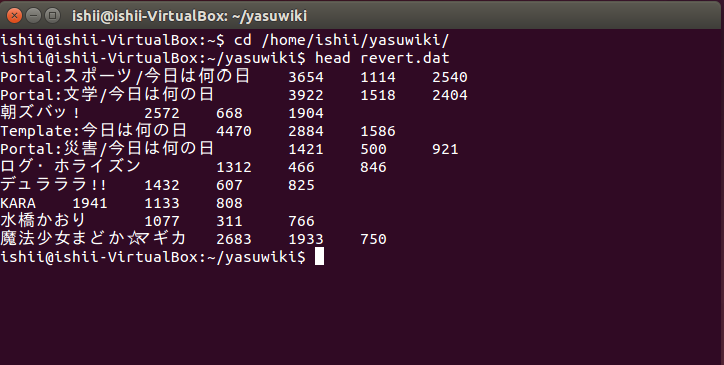
\includegraphics[width=14cm]{head_revert.png}
\caption{差し戻し回数の多いページ}\label{サンプル図}
\end{figure}


%次のページに移動
\clearpage

\subsection{編集者の調査}

「stub-meta-history」の中から,「pageId[tab]revisionId[tab]userId[tab]ip」というデータを作る.詳細は以下のeditors2.pyを参照. \\
\\
editors2.py

{\small
\begin{verbatim}
# -*- coding: utf-8 -*-

import xml.sax
import sys

class myHandler(xml.sax.ContentHandler):
  reading = {"id":False, "contributor":False, "revision":False, "ip":False, "timestamp":False}
  pageId = ""
  revisionId = ""
  userId = ""
  ip = ""
  timestamp = ""

  def __init__(self):
    xml.sax.ContentHandler.__init__(self)

  def startElement(self, name, attrs):
    self.reading[name] = True

  def endElement(self, name):
    self.reading[name] = False
    if name == "page":
      self.pageId = ""
    elif name == "revision":
      print(self.pageId + "\t" + self.revisionId + "\t" + self.userId + "\t" + self.ip + "\t" +
      self.timestamp)
      self.revisionId = ""
      self.userId = ""
      self.ip = ""
      self.timestamp = ""

  def characters(self, content):
    if self.reading["id"] == True:
      if self.reading["contributor"] == True:
        self.userId = self.userId + content
      elif self.reading["revision"] == True:
        self.revisionId = self.revisionId + content
      else:
        self.pageId = self.pageId + content
    elif self.reading["ip"] == True:
        self.ip = self.ip + content

    elif self.reading["timestamp"] == True:
    	self.timestamp = self.timestamp + content

def main():
  xml.sax.parse(sys.stdin, myHandler()) 
if __name__ == "__main__":
  main()
\end{verbatim}}

以下のコマンドを入力した.

{\small
\begin{verbatim}
cat jawiki-20150901-stub-meta-history.xml | python3 editors2.py | less
\end{verbatim}}

結果は以下のとおりである.データとしてとる場合は「| less」の部分を「> editors2.dat」とした. \\


%図の挿入
\begin{figure}[H]
\centering
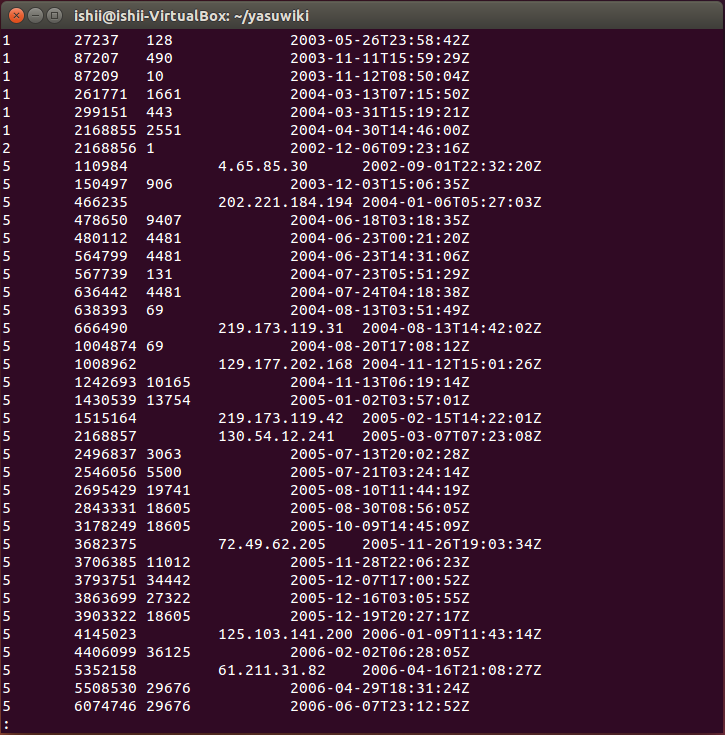
\includegraphics[width=10cm]{editors2_data.png}
\caption{編集者の調査}\label{サンプル図}
\end{figure}


このeditors2.datをmysqlにインポートしたいため,CSV化する.そのため,以下のようにコマンドを入力し,「,」区切りにする.csvファイルでとるときは「| less」の部分を「> editors2.csv」とかする.

{\small
\begin{verbatim}
cat editors2.dat | awk 'BEGIN {FS="";} {print $1","$2","$3","$4","$5}' | less
\end{verbatim}}

結果は以下のとおり,

%図の挿入
\begin{figure}[H]
\centering
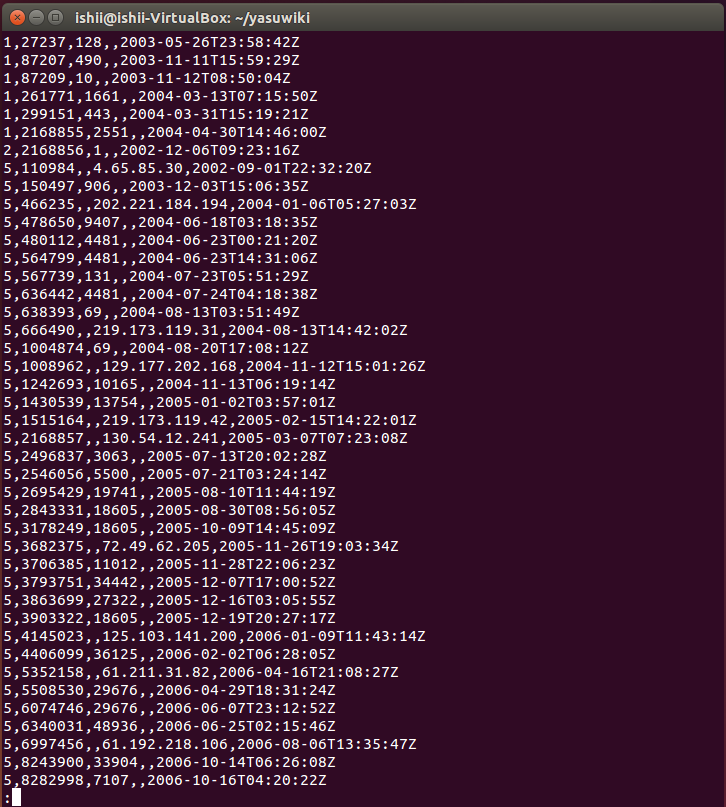
\includegraphics[width=10cm]{editors2_csv.png}
\caption{編集者の調査csv化}\label{サンプル図}
\end{figure}


editors2.csvのuserIdから役割がある人(管理者とかbotとか)たちにroleをつける.

%次のページに移動
\clearpage

詳細はwikipediaが提供しているデータにある「jawiki-latest-user\_groups.sql.gz」を参照する. \\
本研究では「jawiki-20150901-user\_groups.sql.gz」を使用.中身は以下のとおり. 

%図の挿入
\begin{figure}[H]
\centering
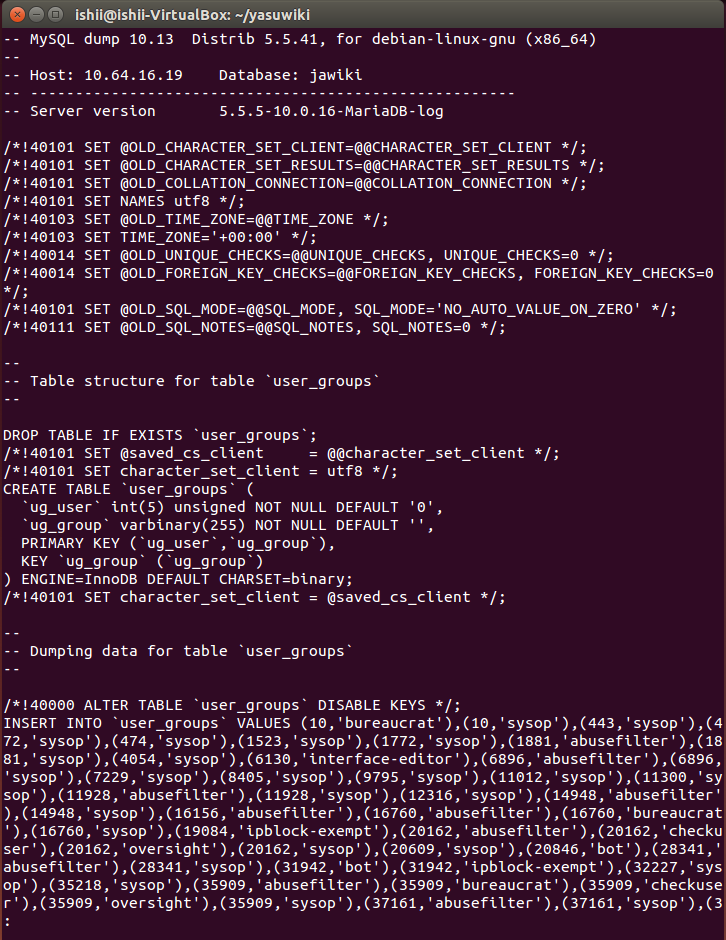
\includegraphics[width=10cm]{user_group1.png}
\caption{ユーザーグループ情報}\label{サンプル図}
\end{figure}


%次のページに移動
\clearpage

\subsection{インポート}

「editors2.csv」と「jawiki-20150901-user\_groups.sql」の,2つのファイルをmysqlへインポートを行う. \\

editors2.pyの場合 \\
\\
ローカル内でmysqlへ接続して行った.\\
まずmysqlで以下のように入力し,「editors」テーブルを作成する.


{\small
\begin{verbatim}
mysql>CREATE TABEL editors(
                       pageId INT NOT NULL,
                       revisionId INT NOT NULL,
                       userId VARCHAR(30) NOT NULL,
                       ip VARCHAR(30) NOT NULL,
                       timestamp TIMESTAMP NOT NULL,
                       KEY (userId)
                      )DEFAULT CHARSET=utf8;
\end{verbatim}}

そして,作成したeditorsテーブルへ「editors2.csv」ファイルをインポートする.以下のように入力する.(この作業には時間がかかる.本研究では3時間ほどかかった.)

{\small
\begin{verbatim}

mysql>LOAD DATA LOCAL INFILE "/home/ishii/yasuwiki/editors2.csv" INTO TABLE editors
         FIELDS TERMINATED BY ',' ENCLOSED BY '"'
         (pageId,revisionId,userId,ip,timestamp);

\end{verbatim}}

インポートが完了したら,以下のように入力し,中身を確認する(LIMITをつけているのはデータ量が膨大なため,全て処理すると時間がかかってしまうから)

{\small
\begin{verbatim}

mysql>SELECT * FROM editors LIMIT 100;

\end{verbatim}}


%次のページに移動
\clearpage

結果はこのようになっていれば終了.

%図の挿入
\begin{figure}[H]
\centering
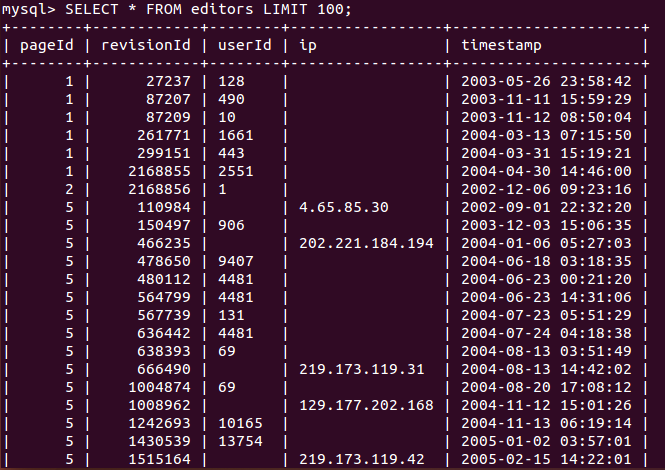
\includegraphics[width=10cm]{editors_table_check.png}
\caption{editorsテーブルの中身を確認}\label{サンプル図}
\end{figure}

jawiki-20150901-user\_groups.sqlの場合\\
\\
phpmyadminからインポートを行った.「usergroups」テーブルを作成する.

以下の画面のように,phpmyadminからインポートのタグに移動する. \\
「インポートするファイル:」の中の,「アップロードファイル:」の参照をクリックする.そして,「jawiki-20150901-user\_groups.sql」を保存した場所から選択する.他は何も変更せずに,下の方にある「実行」ボタンをクリックする.

%図の挿入
\begin{figure}[H]
\centering
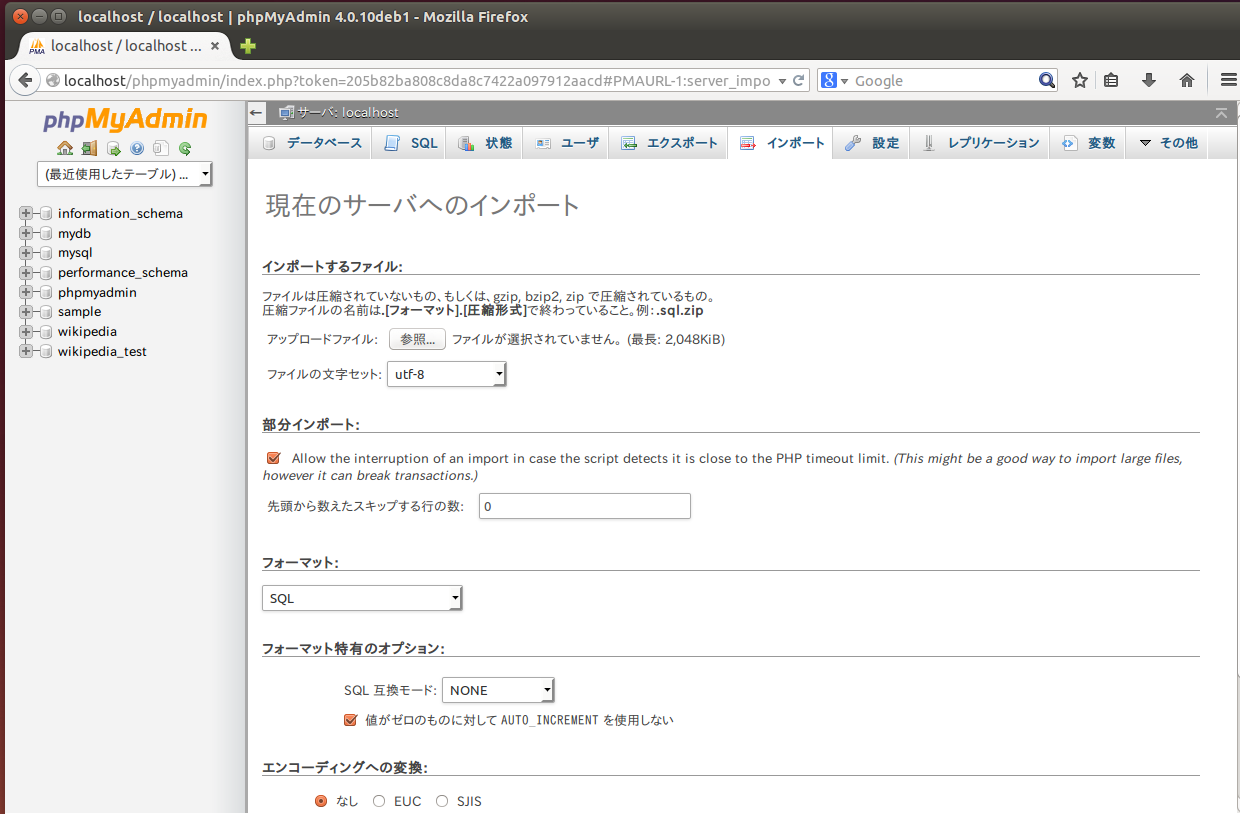
\includegraphics[width=10cm]{inport.png}
\caption{phpmyadminのインポート画面}\label{サンプル図}
\end{figure}




\subsection{外部結合}

インポートした「editors」テーブルと「」テーブルの外部結合を行う.\\
ローカルでmysqlへ接続し,以下を入力する.「userId,ip,ug\_group,timestamp」の入った,「editors\_role」テーブルを作成する.(この作業には時間がかかる.本研究では3時間ほどかかった)


{\small
\begin{verbatim}
mysql>CREATE TABLE editors_role(
         SELECT editors.userId,ip,user_group,timestamp
         FROM editors
         LEFT JOIN user_groups ON editors.userId=user_groups.ug_user
        );
\end{verbatim}}

%図の挿入
\begin{figure}[H]
\centering
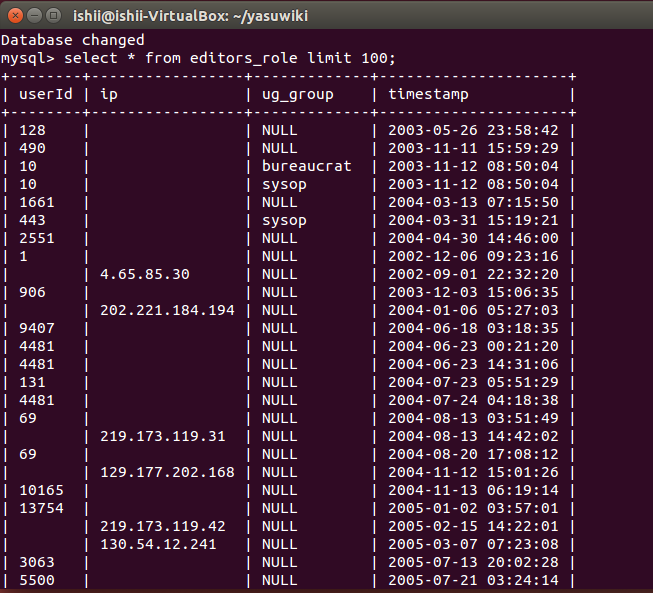
\includegraphics[width=10cm]{editors_role1.png}
\caption{editors\_roleテーブルの中身}\label{サンプル図}
\end{figure}

%次のページに移動
\clearpage


管理者の月別編集の割合を探るので,次にeditors\_roleの中から管理者だけの編集履歴を抽出する.mysql内で以下を入力した.\\
\\
中身は以下のとおりになる.

{\small
\begin{verbatim}
mysql>CREATE TABEL sysop_editors_only(
         SELECT userId,ug_group,timestamp
         FROM editors_role
         WHERE ug_group = 'sysop'
         );
\end{verbatim}}


%図の挿入
\begin{figure}[H]
\centering
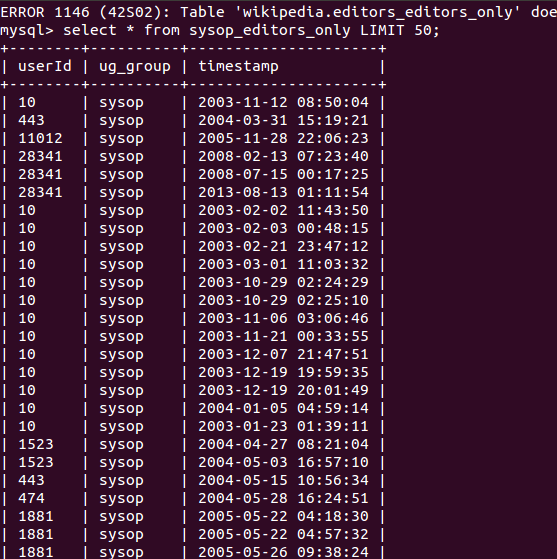
\includegraphics[width=10cm]{sysop_editors_only1.png}
\caption{sysop\_editors\_onlyテーブルの中身}\label{サンプル図}
\end{figure}



%次のページに移動
\clearpage

\subsection{エクスポート}

外部結合して作成したテーブルをエクスポートする.phpmyadmin内で行った.フォーマットの選択肢で「CSV for MS Excel」を選択肢,実行ボタンを押す.保存するファイル名は「sysop\_editors\_only.csv」とした.

%図の挿入
\begin{figure}[H]
\centering
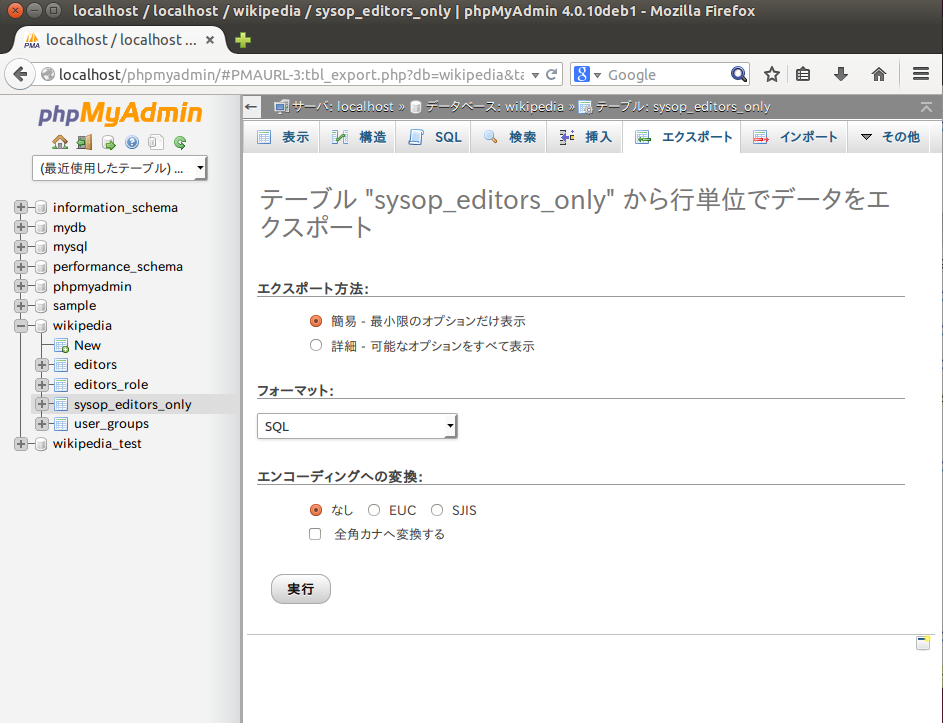
\includegraphics[width=10cm]{sysop_editors_only2.png}
\caption{phpmyadminのエクスポート画面}\label{サンプル図}
\end{figure}


%次のページに移動
\clearpage

\subsection{管理者の月別編集回数}

当研究の作業ディレクトリ内で,以下のコマンドを入力する.

{\small
\begin{verbatim}
cut -d ',' -f 3 sysop_editors_only.csv | cut -c2-8 | sort | uniq -c > sysop_month.dat
\end{verbatim}}

この「sysop\_month.dat」をExcelで(テキスト形式で)読み込めばよいが,次のようにCSV化した方が簡単なので行った.

{\small
\begin{verbatim}
cut sysop_month.dat | awk '{print $2","$1} > sysop_month.csv
\end{verbatim}}




以下が抽出したファイルのデータからグラフ化したものである.

%図の挿入
\begin{figure}[H]
\centering
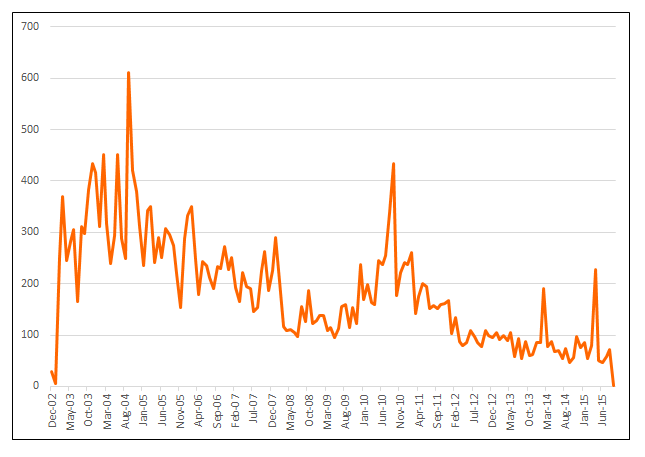
\includegraphics[width=10cm]{sysop_month.png}
\caption{管理者の月別編集回数}\label{サンプル図}
\end{figure}



\subsection{全ての編集履歴の月別編集回数}

編集履歴のデータから,grepでタイムスタンプを取り出し,cutで「西暦-月」を切り出し,sortで並び替え,uniqで集計する。以下のコマンドを入力する.

{\small
\begin{verbatim}
gunzip -c jawiki-20150901-stub-meta-history.xml.gz | grep "<timestamp>" | cut -c18-24 | sort | uniq -c > month.dat
\end{verbatim}}

次にCSV化を行う.

{\small
\begin{verbatim}
cat month.dat | awk '{print $2","$1}' > month.csv
\end{verbatim}}

%次のページに移動
\clearpage

以下が抽出したファイルのデータからグラフ化したものである.

%図の挿入
\begin{figure}[H]
\centering
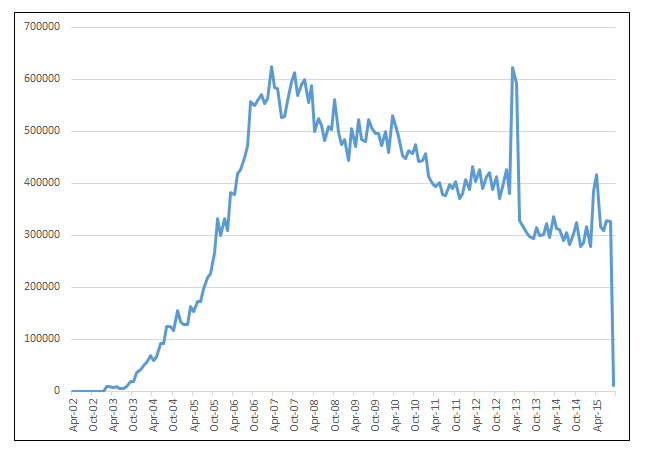
\includegraphics[width=10cm]{month1.png}
\caption{月別編集回数}\label{サンプル図}
\end{figure}


\subsection{総編集回数における管理者の編集の割合}


%図の挿入
\begin{figure}[H]
\centering
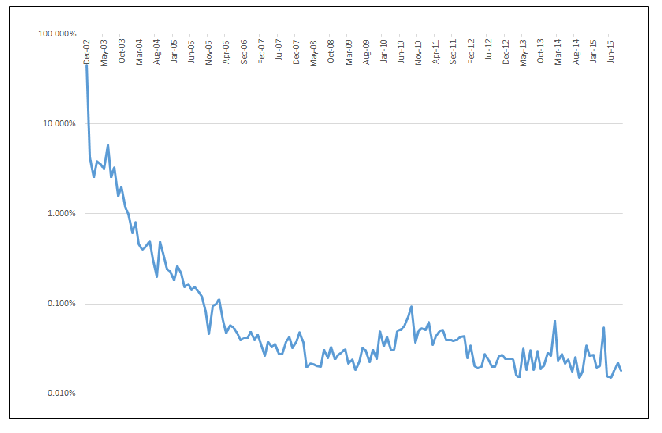
\includegraphics[width=10cm]{sysop_per.png}
\caption{総編集回数における管理者の編集の割合の変化}\label{サンプル図}
\end{figure}

図のような結果になった.編集する割合は年々減少傾向にあった.



%↑ここからスタート





\chapter{考察}

日本語版Wikipedia では,管理者が編集を行う必要性が薄れてきている.実装当初から,管理者は毎月約300~400 回ほどの編集を行っていたが,2015年5 月ごろからは,月に100 回も行わないことが多くなってきているからである.


\chapter{結論}

日本語版Wikipedia では,管理者が編集を行う割合は年々減少している傾向だった.

管理者が不足しているにもかかわらず,プロジェクトが日々動いている要因として,日本人の「礼儀正しさ」が挙げられる.日本の文化は比較的均一なため,用法や言動についての論争があまり生まれない.また日本語版のWikipediaでは,長くて卑劣な論争の編集合戦などは一般的に受け入れられないので,行わない傾向があるからだ.

\bibliographystyle{junsrt}
\bibliography{biblio}%「biblio.bib」というファイルが必要.

\end{document}